\documentclass[a4paper,fleqn]{cas-dc}

\usepackage[authoryear,longnamesfirst]{natbib}
\usepackage{graphicx}
\usepackage{booktabs}
\usepackage{multirow}
\usepackage{tabularx}
\usepackage{array}
\usepackage{pifont}

\newcommand{\xfig}[1]{\hyperref[#1]{Figure~\ref*{#1}}}
\newcommand{\xtab}[1]{\hyperref[#1]{Table~\ref*{#1}}}
\newcommand{\xsec}[1]{\hyperref[#1]{Section~\ref*{#1}}}

\begin{document}
\let\WriteBookmarks\relax
\def\floatpagepagefraction{1}
\def\textpagefraction{.001}

\shorttitle{FPMANR}

\title[mode = title]{FPMANR: An Integrated Framework for Stable, Privacy-Preserving, and Attack-Resistant Federated Learning under Non-IID Data}

\author[1]{Israt Tasnim Esha}[]
\cormark[1]
\ead{israttasnimesha1046@gmail.com}

\affiliation[1]{organization={Department of Computer Science and Engineering, University of Brahmanbaria},
            city={Brahmanbaria},
            country={Bangladesh}}

\cortext[cor1]{Corresponding author}

\begin{abstract}
Federated learning (FL) faces challenges in training stability, privacy, and secure communication, especially under non-IID data across distributed clients. Existing methods typically address optimization, privacy, or secure aggregation separately, but not all three together. This paper proposes FPMANR, an integrated FL framework combining FedProx-based local training, two-neighbor pairwise masking in a ring topology, layer-wise adaptive Gaussian noise, and a client dropout recovery mechanism. In each communication round, 30 of 100 clients with Dirichlet-based non-IID data are selected to train a shared global model using FedProx. Before transmission, each client adds adaptive layer-wise Gaussian noise, where larger updates receive stronger perturbation, followed by pairwise masking with two neighbors. A recovery mechanism handles client dropouts without local retraining. Experiments on EMNIST Digits, EMNIST Letters, and Fashion-MNIST compare four settings: FedProx (FP), FedProx with masking (FPM), and FPMANR with adaptive noise factors of 0.1 and 0.2 (FPMANR 0.1 and FPMANR 0.2). Results show the expected privacy--utility trade-off, where adaptive noise improves privacy with only moderate accuracy reduction. FPMANR 0.1 achieves test accuracies of 98.10\% on EMNIST Digits, 85.39\% on EMNIST Letters, and 74.51\% on Fashion-MNIST. Quantitative evaluation using MSE, PSNR, SSIM, LPIPS, and reconstruction success rate demonstrates substantially stronger resistance to DLG, iDLG, and GradInv attacks. Membership inference attacks remain close to random guessing, with AUC values around 0.5 and attack accuracy near 50\%. Overall, FPMANR provides a practical and attack-resistant FL framework with stable training, improved privacy, and dropout resilience under heterogeneous data settings.
\end{abstract}

\begin{keywords}
federated learning \sep non-IID data \sep pairwise masking \sep adaptive Gaussian noise \sep gradient reconstruction attacks \sep membership inference attacks
\end{keywords}

\maketitle

\section{Introduction}
\label{sec:1}

In traditional centralized machine learning (ML), data from multiple sources is transferred to a central server, where a global model is trained using the aggregated dataset \citep{majeed2022comparative}. However, centralizing data raises regulatory, ethical, legal, and technical challenges related to privacy and data protection, since anonymized electronic health records that appear GDPR- or PHI-compliant may still allow patient re-identification and information leakage \citep{rieke2020future}. Moreover, centralized training incurs significant communication overhead and increased training time due to continuous data and parameter transmission between clients and the central server \citep{thangavel2023distributed}. Federated learning (FL) addresses these limitations by reducing communication cost and network congestion caused by frequent data transfers in centralized learning settings \citep{mcmahan2017communication}. FL enables collaborative model training across multiple participants without sharing raw data, thereby improving model generalization while preserving data privacy \citep{mammen2021federated}. However, FL still faces challenges under non-IID data distributions \citep{xiong2021privacy} and remains vulnerable to gradient reconstruction attacks \citep{guo2025exploring} and membership inference attacks (MIAs) \citep{bai2024membership}.

FL algorithms such as FedProx mitigate non-IID data effects by adding a proximal term to stabilize local training and improve convergence \citep{cao2025comparative}. Differential Privacy (DP) is widely used in FL to protect user privacy by adding noise to model parameters before sharing them with the server \citep{nilsson2018performance}. This privacy protection may come at the cost of reduced model performance due to the injected noise \citep{zhang2021survey}. Adaptive Gaussian noise has been proposed to enhance privacy protection while reducing the performance degradation caused by fixed-noise differential privacy mechanisms \citep{jiao2023differential}. Secure aggregation has been introduced in FL to hide individual client updates from the server using cryptographic masking, but it does not fully prevent membership inference or data reconstruction attacks in practice \citep{bonawitz2017practical}. Existing approaches address different aspects of FL such as non-IID data handling, privacy preservation, communication efficiency, and robustness against inference and reconstruction attacks, but no single method fully resolves all these challenges together. This leaves a gap in designing FL frameworks that combine stable training under heterogeneous data, adaptive privacy for sensitive layers, and secure transmission of updates while maintaining acceptable model accuracy.

To address these challenges, FPMAN was initially proposed in \citet{esha2026fpman} as an integrated FL framework combining FedProx, pairwise masking, and layer-wise adaptive Gaussian noise for stable and privacy-preserving learning under non-IID data. This paper, referred to as FPMANR, further formalizes and evaluates a client dropout recovery procedure inherent to the masking design, and extends the evaluation with broader experiments across multiple datasets and additional privacy attack analysis.

The main contributions of this study are summarized as follows:

\begin{enumerate}
\item
  FedProx improves convergence stability under highly non-IID client data distributions.
\item
  A two-neighbor pairwise masking scheme in a ring topology protects client updates while preserving correct aggregation with low communication overhead.
\item
  A dropout recovery procedure, formalized and evaluated for the first time in this work, ensures correct aggregation under client failures without local retraining.
\item
  Layer-wise adaptive Gaussian noise perturbs updates based on magnitude, improving privacy--utility balance.
\item
  Experiments on EMNIST Digits, EMNIST Letters, and Fashion-MNIST evaluate FP, FPM, FPMANR 0.1, and FPMANR 0.2, showing that FPMANR 0.1 achieves the best privacy--utility trade-off with high accuracy across datasets.
\item
  DLG, iDLG, GradInv, and MIAs show that FPMANR significantly reduces gradient reconstruction and reduces membership inference accuracy to near random level.
\item
  FPMANR integrates FedProx, pairwise masking, adaptive noise, and dropout recovery into a unified framework for secure and robust FL.
\end{enumerate}

The remainder of this paper is organized as follows. \xsec{sec:2} reviews related works on FL and privacy techniques. \xsec{sec:3} presents the preliminaries required for this study. \xsec{sec:4} describes the proposed FPMANR methodology. \xsec{sec:5} introduces the threat model considered in this work. \xsec{sec:6} presents the performance analysis, including experimental setup, results, attack analysis, and comparison with existing methods. \xsec{sec:7} concludes the paper.

\section{Related Works}
\label{sec:2}

The foundation of FL was established by McMahan et al. with FedAvg \citep{mcmahan2017communication}, enabling decentralized training via local SGD and global model averaging. FedAvg achieves similar target accuracy under IID and non-IID settings (e.g., 99\% MNIST, 54\% Shakespeare), but requires far more communication rounds under non-IID data ($\approx$18--65 vs. 173--600 on MNIST CNN), showing degraded convergence due to client drift and data heterogeneity. FedProx \citep{li2020federated} extends FedAvg by introducing a proximal term in the local objective and allowing partial local updates to handle device and data heterogeneity. It is evaluated on Synthetic($\alpha$,$\beta$), MNIST, FEMNIST, Shakespeare, and Sent140 datasets under federated non-IID settings. Compared to FedAvg, FedProx improves stability under high heterogeneity, achieving up to \textasciitilde22\% higher test accuracy in highly non-IID and straggler-heavy scenarios (e.g., 90\% stragglers), while preventing divergence and maintaining convergence where FedAvg becomes unstable. FedProx \citep{dai2024comparative} is further shown to outperform FedAvg, FedSGD, and SCAFFOLD on non-IID Fashion-MNIST using a CNN under identical settings (5 clients, 10 rounds). It achieves the highest performance with 91.59\% accuracy (vs. 89.95\% FedAvg, 89.98\% SCAFFOLD, 79.43\% FedSGD) along with superior precision, recall, and F1-score. The improvement is due to its proximal term, which reduces client drift under heterogeneous data, leading to more stable and consistent convergence across clients. However, FedProx does not inherently prevent gradient inversion or MIAs, as it still transmits model updates/gradients without explicit privacy protection, making it vulnerable to inference-based privacy attacks similar to FedAvg.

DP-SGD \citep{fernandez2025differential} addresses this privacy limitation by mitigating gradient reconstruction attacks in FL. On MNIST and Food-101-based CNN experiments, non-DP training enables near-perfect gradient inversion (SSIM $\approx$ 1), whereas DP-SGD successfully destroys reconstruction quality, producing noise-like outputs with very low similarity to the original data, while PDP-SGD fails to provide such protection and still allows recognizable reconstruction. Bayesian DP (BDP) \citep{nguyen2023active} further improves privacy guarantees against inference-based attacks such as MIAs by providing tighter $\epsilon$-bounds through Bayesian accounting. Lower $\epsilon$ ($\approx$1 for clients, $\approx$0.1 for instance-level DP) strengthens worst-case protection and reduces the theoretical success probability of membership inference compared to standard DP. However, Bayesian DP \citep{triastcyn2019federated} shows that stronger privacy often comes at the cost of model utility. Although BDP reduces the privacy budget to about $\epsilon$$\approx$1 for client-level and $\epsilon$$\approx$0.1 for instance-level privacy, standard DP can suffer severe accuracy degradation under strong protection (e.g., from 97\% to 12\% on non-IID MNIST), while even BDP retains only 62\% accuracy. This highlights the persistent challenge of balancing strong privacy with model performance in FL.

Adap DP-FL \citep{fu2022adap} addresses the privacy--utility trade-off of conventional DP by introducing adaptive gradient clipping and adaptive noise scheduling instead of fixed privacy parameters. Under the same privacy budget ($\epsilon$ = 2, $\delta$ = 10$^{-5}$), it improves the performance of standard DP-FL, achieving 94.15\% accuracy on MNIST and 79.56\% on Fashion-MNIST while maintaining the same formal differential privacy guarantees. Adaptive DP survival framework \citep{niu2025adaptive} further extends this direction by introducing layer-sensitive adaptive DP allocation in federated survival analysis. Compared with standard DP, it improves C-index from 0.5843--0.6508 to 0.6276--0.6698 under $\epsilon$ = 1--3, achieving gains up to +0.0433 while preserving the privacy--utility trade-off.

LDP-Fed \citep{truex2020ldp} shifts the setting from global DP to local differential privacy, where clients perturb updates before transmission. Using top-k selection with bounded noise and budget allocation, it achieves up to 95.21\% accuracy on MNIST and 82.20\% on Fashion-MNIST, improving over standard LDP baselines by 3--9\%, while significantly reducing communication cost by up to 95\% through sparse updates. However, strong privacy budgets still reduce accuracy, especially under small-scale client settings. ALDP-FL \citep{cui2025aldp} further improves this local privacy direction by introducing layer-wise adaptive clipping and bounded perturbation, reducing unnecessary noise while strengthening attack resistance. With local privacy parameters ($\epsilon$ = 4, $\delta$ = 10$^{-7}$), it improves accuracy by 3--13\%, reduces SSIM by \textasciitilde85\%, and increases reconstruction error (MSE) by \textasciitilde391\% compared with FedAvg.

Secure aggregation methods \citep{bonawitz2017practical} address the privacy--utility limitation of DP-based FL by replacing noise injection with pairwise masking so that only aggregated updates are revealed. The CCS 2017 protocol achieves secure sum computation with about 1.73$\times$--1.98$\times$ communication overhead and preserves exact model accuracy since masks cancel perfectly, but it introduces O(n$\cdot$m) communication cost due to large-scale key exchange, where each client forms pairs with all other clients. GVSA \citep{zhou2025group} improves efficiency of masking-based aggregation by introducing group-based communication, where each client interacts only with other clients inside its group (for example, 9 peers in a 10-user group), reducing communication cost and achieving only \textasciitilde7\% overhead over FedAvg, while being 2.3$\times$ faster than prior secure aggregation schemes with near-identical accuracy (0.888 vs. 0.885 on MNIST). However, these masking-based secure aggregation methods do not fully prevent membership inference or reconstruction-style attacks, since aggregated model updates can still leak information through repeated observations across training rounds.

FPMANR addresses the limitations of both DP-based and masking-based secure aggregation by combining FedProx-based local training, adaptive Gaussian noise, and pairwise masking in a ring structure, where each client exchanges masks with two neighboring clients before sending updates. Unlike masking-based methods \citep{bonawitz2017practical,cui2025aldp}, which use large-scale pairwise or group-based communication, FPMANR uses only two-neighbor masking in a simple ring topology, reducing communication complexity. At the same time, unlike LDP-based methods \citep{niu2025adaptive,truex2020ldp}, which rely only on noise injection and may reduce accuracy under strict privacy settings, FPMANR applies layer-wise adaptive noise based on update magnitude to reduce information leakage while preserving model utility. This combination of masking and adaptive noise improves privacy protection against gradient leakage while maintaining stable performance in non-IID FL.

\section{Preliminaries}
\label{sec:3}

\subsection{Federated Learning (FL)}

FL is a distributed learning approach where multiple clients collaboratively train a global model without sharing their local data, thereby preserving privacy. Each client performs local training on its own dataset and transmits only model updates (e.g., gradients or parameters) to a central server, which aggregates them to update the global model \citep{wen2023survey}. This reduces data leakage risks while enabling learning across decentralized and non-IID data sources. However, FL still faces challenges such as communication cost, data heterogeneity, and privacy attacks on shared updates.

\subsection{Non-IID Data in FL}

In FL, data across clients is typically non-independent and identically distributed (non-IID), as each client collects data from different users or environments, leading to heterogeneous data distributions. This data heterogeneity causes challenges in training, often resulting in slower convergence and reduced model performance. Non-IID data can appear in different forms, including label skew, feature skew, and variations in data quantity across clients, where the underlying joint distribution P(x,y) differs among clients \citep{li2022federated}.

\subsection{FedProx}

FedProx (Federated Proximal) is an extension of FedAvg designed to handle system and data heterogeneity in FL. It introduces a proximal term in the local objective, which restricts each client's model from drifting too far from the global model, making training more stable under non-IID and partial device participation \citep{li2020federated}. Unlike FedAvg, it allows variable local computation across clients without dropping slow devices, improving robustness in heterogeneous environments. This leads to more stable convergence and better performance in practical federated settings.

\subsection{Gradient Reconstruction Attacks}

Gradient reconstruction attacks aim to recover private training data from shared gradients in FL by matching dummy-generated gradients with the real gradients received from clients. Deep Leakage from Gradients (DLG) reconstructs both data and labels through iterative optimization by minimizing gradient difference, while Improved DLG (iDLG) simplifies the process by directly inferring true labels from gradients in single-batch settings. Gradient Inversion with Total Variation (GradInv) further improves reconstruction quality using total variation and regularization terms, making it effective for higher-resolution images and larger batch sizes \citep{zhang2022survey}. These attacks show that shared gradients can still leak sensitive training information in standard FL systems.

To evaluate reconstruction quality, Peak Signal-to-Noise Ratio (PSNR), Structural Similarity Index Measure (SSIM), and Learned Perceptual Image Patch Similarity (LPIPS) are used to measure visual, structural, and perceptual similarity between original and reconstructed images \citep{carletti2026guide}, while Mean Squared Error (MSE) measures the pixel-level reconstruction error \citep{shi2024dealing}. Attack Success Rate (ASR) is used to quantify the percentage of successful reconstructions based on predefined reconstruction quality criteria \citep{he2025crafting}.

\subsection{Membership Inference Attack (MIA)}

MIA aim to infer whether a specific sample was used in training by exploiting differences in model outputs for training and non-training data, often due to model overfitting. In FL, an adversary can observe model updates or query the global model and use shadow models to learn this membership signal without accessing raw data. The attack is typically framed as a binary classification problem that distinguishes ``in'' and ``out'' samples based on model responses \citep{banerjee2023mia}. This makes it possible to leak participation information from client datasets even when data is not directly shared.

To evaluate the effectiveness of MIAs, Confidence Area Under the Curve (Confidence AUC), Loss Area Under the Curve (Loss AUC), Entropy Area Under the Curve (Entropy AUC), and Attack Accuracy are commonly used. These metrics measure the attacker's ability to distinguish training samples from non-training samples based on model confidence, prediction loss, entropy, and classification performance, respectively \citep{shokri2017membership}. Lower values indicate stronger privacy protection against MIAs.

\section{Methodology}
\label{sec:4}

This section presents the involved entities and the individual stages of the proposed framework. \xfig{fig:1} illustrates the overall architecture of the proposed system.

\begin{figure*}
\centering
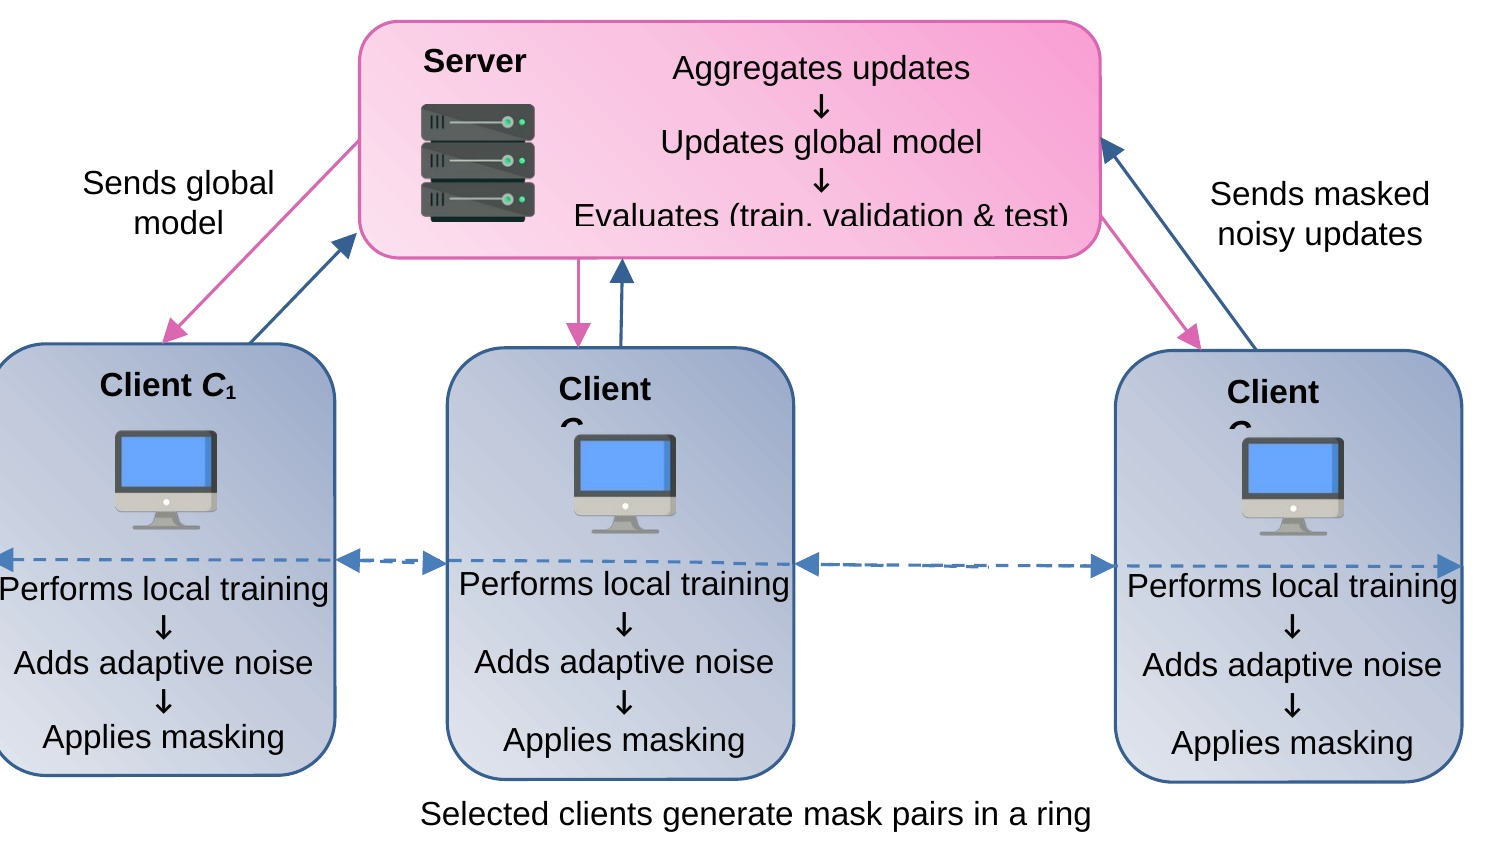
\includegraphics[width=0.8\textwidth]{figures/fig1_architecture.jpg}
\caption{Architecture of the proposed framework.}
\label{fig:1}
\end{figure*}

\subsection{Involved Entities}

The proposed framework consists of two main entities: a central server and multiple clients.

\textbf{Server:} The server initializes the global model and coordinates the federated training process. During each communication round, it selects participating clients and distributes the current global model $\theta_{G}$ to them. It receives the masked client updates, aggregates them to compute the average update, and updates the global model accordingly. The server also evaluates the updated model using training, validation and test datasets.

\textbf{Clients:} Each client stores its own private local dataset $d_{i}$, following a non-IID data distribution. When selected for a communication round, a client receives the global model $\theta_{G}$, performs local training using FedProx, and computes the local update $\Delta_{i}$. Before transmission, the client applies adaptive noise and pairwise masking with two neighboring clients to protect the update. Clients keep their raw local data and original updates private, and transmit only the masked updates to the server.

\subsection{Individual Stages}

This section presents the FL setup, including the datasets, client distribution strategy, local training process, privacy protection mechanism, and global model aggregation procedure. It describes how non-IID data is distributed among clients, how local model updates are generated and protected using masking and adaptive noise, and how the server aggregates the received updates to train the global model.

\subsubsection{Data Collection and Preparation}
\label{sec:4.2.1}

The experiments are conducted using three benchmark image classification datasets: EMNIST Digits \citep{cohen2017emnist}, EMNIST Letters \citep{cohen2017emnist}, and Fashion-MNIST \citep{xiao2017fashion}. All datasets contain grayscale images with a resolution of 28 $\times$ 28 pixels and are widely used for evaluating ML and FL models. In all experiments, the training sets are distributed among clients for FL, while the test sets are used to evaluate the performance of the global model. The learning task is formulated as a multi-class image classification problem, where the model predicts the correct class label for each input image.

The EMNIST Digits dataset is a benchmark dataset for handwritten digit recognition. It contains images of digits from 0 to 9 collected from different writers. The dataset includes 240,000 training images and 40,000 test images distributed across 10 classes. Due to variations in handwriting styles, the dataset provides a realistic and challenging environment for evaluating classification performance.

The EMNIST Letters dataset is designed for handwritten letter recognition. It contains grayscale images of English alphabet letters represented in 26 balanced classes. The dataset includes 124,800 training images and 20,800 test images. Compared to digit recognition, letter classification is more challenging because of the visual similarity between several handwritten characters.

The Fashion-MNIST dataset is a widely used benchmark dataset for image classification. It consists of grayscale images of fashion products such as shirts, trousers, shoes, bags, and coats. The dataset contains 60,000 training images and 10,000 test images divided into 10 categories. Compared to handwritten digit datasets, Fashion-MNIST contains more detailed visual patterns and greater inter-class similarity, making the classification task comparatively more challenging.

\subsubsection{Dataset and Client Distribution}
\label{sec:4.2.2}

The training dataset is distributed among 100 clients using a Dirichlet-based non-IID partitioning strategy. The client data distribution is generated using a Dirichlet distribution with concentration parameter $\beta = 0.1$, producing highly skewed, imbalanced, and heterogeneous local datasets across clients. Consequently, each client contains samples from only a subset of classes, creating a strict non-IID FL setting. Formally, the dataset $D$ is partitioned into client-specific local datasets as $D \rightarrow \left\{ d_{1}, d_{2}, \ldots, d_{100} \right\}$, where each client $j$ privately stores its local dataset $d_{j}$ throughout the FL process.

Among the 100 clients, 10 fixed clients are reserved exclusively for validation and do not participate in local training. During each communication round, 30 clients (30\% of the total clients) are randomly selected from the remaining 90 training clients to perform local model updates, while the remaining clients stay inactive for that round.

A unified Convolutional Neural Network (CNN) architecture is used across all clients and the central server for all datasets. The model consists of two convolutional layers with 3$\times$3 kernels and 32 and 64 feature maps, respectively, each followed by ReLU activation and 2$\times$2 max-pooling for spatial down-sampling. The resulting feature representations are flattened and passed through a fully connected layer with 256 neurons using ReLU activation, followed by a final output layer that produces logits. The output dimension is dataset-dependent, corresponding to 10 classes for EMNIST Digits and Fashion-MNIST, and 26 classes for EMNIST Letters.

\subsubsection{Local Update Computation}
\label{sec:4.2.3}

At the beginning of training, the server initializes the global model with random parameters $\theta_{G}$. In each communication round, the server randomly selects 30 out of 90 training clients and sends the current global model $\theta_{G}$ to them.

Each selected client $C_{j}$ trains the received global model on its local dataset $d_{j}$ using the FedProx framework, which stabilizes training under non-IID settings by restricting the deviation of the local model from the global model. The local loss function is defined as:

\begin{equation}
L_{j} = \frac{1}{B} \sum_{(x, y) \in \mathrm{batch}}{\mathrm{CrossEntropy}\left( \mathrm{model}(x),y \right)} + \frac{\mu}{2} \sum_{k = 1}^{K}\left\| \theta_{j}^{k} - \theta_{G}^{k} \right\|^{2}
\label{eq:1}
\end{equation}

where $x$ denotes the input, $y$ its corresponding label, $B$ is the batch size, $\mu$ is the proximal term coefficient, $k = 1\ldots K$ indexes all layers or parameter tensors, $\theta_{j}^{k}$ represents client $C_{j}$'s parameters for layer $k$, and $\theta_{G}^{k}$ represents the corresponding global parameters. The first term corresponds to the standard cross-entropy loss, while the second term penalizes deviation of local parameters from the global model.

After local training, each client computes its model update relative to the global model as:

\begin{equation}
\Delta_{j} = \theta_{j} - \theta_{G}
\label{eq:2}
\end{equation}

where $\theta_{j}$ denotes the locally trained model of client $C_{j}$, and $\Delta_{j}$ represents the change in all model parameters induced by its local training process.

\subsubsection{Privacy Protection with Masking and Adaptive Noise}
\label{sec:4.2.4}

If a client directly transmits its raw update $\Delta_{j}$ to the server, the server may infer sensitive information about the client's local data distribution, such as dominant classes or approximate input patterns. To mitigate this risk, cryptographic masking is applied, where each client $C_{j}$ generates pairwise random masks with its two neighboring clients in a ring structure and applies them to its local model update.

However, masking alone cannot provide complete privacy protection. Although the server cannot directly observe individual updates, the update $\Delta_{j}$ may still contain information about the client's local data. For instance, large parameter values in $\Delta_{j}$ usually indicate that the client has many samples of a certain class or pattern. Therefore, some information about the local data may still be inferred even after masking.

Privacy leakage may also occur if neighboring clients are compromised or collude with an attacker. Since each mask is shared between two clients, a malicious neighbor may reveal its mask values, partially exposing the masked update. This shows that masking alone is not sufficient to completely hide sensitive information.

To further reduce this privacy risk, small adaptive Gaussian noise is first added to each layer of the local update before any masking operation. The noise magnitude is controlled by the Adaptive Noise Factor (ANF), denoted by $\alpha$. For client $C_{j}$ and layer $l$, the noisy update is defined as:

\begin{equation}
\Delta_{j}^{l, \mathrm{noisy}} = \Delta_{j}^{l} + n_{j}^{l}
\label{eq:3}
\end{equation}

where $n_{j}^{l}$ represents a Gaussian noise vector added element-wise to all parameters of layer $l$. The noise has zero mean, and its standard deviation is proportional to the norm of the layer update: $\sigma_{l} = \alpha\left\| \Delta_{j}^{l} \right\|_{2}$, where $\alpha > 0$ controls the noise magnitude, and $\alpha = 0$ indicates that no noise is added. The overall noisy update $\Delta_{j}^{noisy}$ is obtained by combining all layer-wise noisy updates $\Delta_{j}^{l, noisy}$ over all model parameters. Each client temporarily stores $\Delta_{j}^{noisy}$ during the communication round until the server confirms successful aggregation or triggers a recovery procedure.

Adding adaptive noise slightly perturbs the model updates. Excessive noise may reduce model accuracy and increase training loss. By scaling the noise according to the norm of each layer update, layers with larger updates, which may reveal more information about the client's local data, receive proportionally larger noise, while layers with smaller updates receive less noise. This adaptive strategy improves privacy protection while minimizing unnecessary performance degradation. Unlike conventional differential privacy methods that apply uniform noise to all layers, the proposed approach better preserves model accuracy and training stability.

Small ANFs of $\alpha = 0.1$ and $\alpha = 0.2$ are considered to balance privacy protection and model utility across the EMNIST Digits, EMNIST Letters, and Fashion-MNIST datasets. An $\alpha$ value of 0.1 introduces mild perturbation that is sufficient to reduce information leakage while maintaining high accuracy and low loss. A moderate $\alpha$ of 0.2 applies stronger noise to further improve privacy protection, although it leads to a larger reduction in model performance. Thus, increasing $\alpha$ generally strengthens privacy at the cost of accuracy and training stability. Although the proposed approach reduces information leakage, it does not provide a formal differential privacy guarantee.

In the proposed framework, the combination of FedProx, pairwise masking, adaptive noise, and dropout recovery is referred to as FPMANR. While small adaptive noise alone provides limited privacy protection, pairwise masking already conceals individual client updates during transmission. The addition of adaptive noise further reduces information leakage with only minor modification to the updates. Moderate noise levels improve privacy protection while maintaining relatively stable model accuracy and loss.

In each communication round, the server constructs a ring structure only among the selected clients and assigns two neighbors to each participating client $C_{j}$, namely client $C_{i}$ (left) and client $C_{k}$ (right). For each neighboring pair, pairwise masks satisfy

\begin{equation}
M_{ij} = - M_{ji}, \quad M_{jk} = - M_{kj}
\label{eq:4}
\end{equation}

where $M_{ji}$ and $M_{ij}$ are the pairwise masks shared between client $C_{j}$ and client $C_{i}$, and $M_{jk}$ and $M_{kj}$ are the pairwise masks shared between client $C_{j}$ and client $C_{k}$.

After adding adaptive noise, client $C_{j}$ forms its masked update as:

\begin{equation}
{\widetilde{\Delta}}_{j}^{noisy} = \Delta_{j}^{noisy} - M_{ji} + M_{jk}
\label{eq:5}
\end{equation}

The resulting noisy and masked update ${\widetilde{\Delta}}_{j}^{noisy}$ is then sent to the server, while keeping each client's individual update private.

\subsubsection{Client Dropout Handling and Recovery}
\label{sec:4.2.5}

In practical FL systems, some selected clients may become unavailable due to communication failures or device interruptions. Since FPMANR uses pairwise masking, client dropouts may prevent proper mask cancellation during aggregation. To address this, a recovery mechanism is introduced to ensure correct aggregation. The recovery mechanism uses the temporarily stored noisy update $\Delta_{j}^{noisy}$ generated in \xsec{sec:4.2.4}, and local retraining is not required during recovery.

\paragraph{Dropout Before Pairwise Mask Generation}
A selected client may become unavailable before establishing pairwise masks with its neighboring clients. Let client $C_{j}$ be paired with clients $C_{i}$ and $C_{k}$. If $C_{j}$ fails to respond during mask establishment, the neighboring clients detect the missing connection and notify the server. The server removes $C_{j}$ from the set of selected clients and instructs $C_{i}$ and $C_{k}$ to establish a direct pairwise connection and generate a new pairwise mask such that

\begin{equation}
M_{ik} = - M_{ki}
\label{eq:6}
\end{equation}

After this reconfiguration, the training process continues normally.

\paragraph{Dropout After Mask Generation but Before Update Transmission}
Let $C_{i}$, $C_{j}$, and $C_{k}$ be three consecutive clients in the pairwise masking ring, where $C_{j}$ is paired with neighboring clients $C_{i}$ and $C_{k}$. A client $C_{j}$ may generate pairwise masks but fail before sending its masked update to the server. In this case, the server receives no update from client $C_{j}$.

Since the updates of $C_{i}$ and $C_{k}$ contain pairwise masks associated with the dropped client $C_{j}$, these masks cannot be canceled during aggregation. Therefore, the server discards the affected updates from $C_{i}$ and $C_{k}$ and initiates a repair procedure.

The repair procedure is as follows:

\begin{enumerate}
\item
  The affected clients $C_{i}$ and $C_{k}$ discard their previously computed masked updates,
\item
  Remove the masks associated with the dropped client $C_{j}$,
\item
  Establish a direct pairwise connection between $C_{i}$ and $C_{k}$ and generate a new pairwise mask,
\item
  Apply the newly generated pairwise mask and the remaining valid pairwise mask to their original noisy updates,
\item
  Resend the repaired masked updates to the server.
\end{enumerate}

After recovery, aggregation proceeds using only the successfully received updates.

\paragraph{Dropout After Update Transmission with Neighbor Failure}
A client $C_{j}$ may successfully transmit its masked update to the server and subsequently drop out, but one of its neighboring clients may fail before transmitting its own update. Consider five consecutive clients $C_{h}$, $C_{i}$, $C_{j}$, $C_{k}$, and $C_{l}$, where $C_{j}$ is paired with $C_{i}$ and $C_{k}$.

If either neighboring client $C_{i}$ or $C_{k}$ fails before transmitting its update, the pairwise masks associated with the failed client cannot be canceled correctly during aggregation. Although the server has already received the masked update of $C_{j}$, client $C_{j}$ is no longer available to participate in the repair process and generate a new mask configuration. Therefore, the server discards the previously received masked update of $C_{j}$ together with the affected neighboring masked updates and initiates a repair procedure.

The repair procedure is as follows:

\begin{enumerate}
\item
  The affected active clients discard their previously computed masked updates,
\item
  Remove the masks associated with the failed clients,
\item
  Establish a new pairwise connection with the nearest active client,
\item
  If $C_{i}$ fails, establish a direct pairwise connection between $C_{h}$ and $C_{k}$ and generate a new pairwise mask,
\item
  If $C_{k}$ fails, establish a direct pairwise connection between $C_{i}$ and $C_{l}$ and generate a new pairwise mask,
\item
  Apply the newly generated pairwise mask together with the remaining valid pairwise masks to their original noisy updates,
\item
  Resend the repaired masked updates to the server.
\end{enumerate}

After recovery, aggregation proceeds using only the active clients that successfully transmit their repaired updates.

\paragraph{Multiple Consecutive Client Dropouts}
If several neighboring clients become inactive during the same communication round, the server skips the inactive clients and connects the nearest active neighbors.

Assume that clients ($C_{p}$, $C_{p+1}$, \ldots, $C_{q}$) become inactive. Since the pairwise masks associated with the inactive clients cannot be canceled during aggregation, the server discards the previously received masked updates affected by the inactive clients. The corresponding active clients remove the masks associated with the inactive clients and discard their previously computed masked updates.

The server then instructs the nearest active clients $C_{p-1}$ and $C_{q+1}$ to establish a direct pairwise connection and generate a new pairwise mask. The affected active clients, whose masked updates contain pairwise masks associated with the inactive clients, apply the newly generated mask together with their remaining valid masks to their original noisy updates and resend the repaired masked updates to the server.

This nearest-active-neighbor recovery mechanism preserves the masking structure while minimizing protocol interruption. Aggregation is performed using only the active clients that successfully transmit their repaired updates.

\paragraph{Aggregation and Recovery Threshold}
After the recovery process, global aggregation is performed only over the active clients. If additional client failures occur during recovery, the server repeats the repair procedure. However, if the number of active clients falls below the predefined threshold of 20, the communication round is aborted and a new client selection process is initiated. The recovery process is performed within the current communication round and does not affect previously completed rounds.

\subsubsection{Global Model Aggregation and Update}
\label{sec:4.2.6}

Once all selected clients have transmitted their noisy and masked updates ${\widetilde{\Delta}}_{j}^{noisy}$, the server performs weighted averaging over the received updates. Let $S$ denote the set of selected active clients in the current communication round, where $n_{j}$ represents the number of data samples at client $C_{j}$, and $n_{k}$ denotes the number of data samples at any client $C_{k} \in S$. The server computes the weighted average update as:

\begin{equation}
\Delta_{avg} = \sum_{j \in S}{\frac{n_{j}}{\sum_{k \in S}n_{k}} {\widetilde{\Delta}}_{j}^{noisy}}
\label{eq:7}
\end{equation}

Because each client $C_{j}$ shares pairwise masks $M_{ji}$ and $M_{jk}$ with its neighboring clients, these masks cancel each other out when summed over all selected clients:

\begin{equation}
\sum_{j \in S}{\left( - M_{ji} + M_{jk} \right) = 0}
\label{eq:8}
\end{equation}

As a result, the weighted average remains unchanged compared to the case without masking:

\begin{equation}
\Delta_{avg} = \sum_{j \in S}{\frac{n_{j}}{\sum_{k \in S}n_{k}} \Delta_{j}^{noisy}}
\label{eq:9}
\end{equation}

Thus, the server only observes the weighted aggregation of the clients' noisy updates, while the individual updates are kept private.

The server then updates the global model as:

\begin{equation}
\theta_{G}^{new} = \theta_{G}^{old} + \Delta_{avg}
\label{eq:10}
\end{equation}

After each communication round, the updated global model is evaluated using cross-entropy loss and classification accuracy. The same evaluation procedure is applied to the training, validation, and test datasets. The cross-entropy loss is defined as:

\begin{equation}
L_{eval} = \frac{1}{\left| D_{eval} \right|} \sum_{(x, y) \in D_{eval}}{\mathrm{CrossEntropy}\left( f_{\theta_{G}}(x),y \right)}
\label{eq:11}
\end{equation}

and the accuracy is computed as:

\begin{equation}
\mathrm{Acc} = \frac{1}{\left| D_{eval} \right|} \sum_{(x, y) \in D_{eval}}{\mathbb{1}\left(\arg\max f_{\theta_{G}}(x) = y\right)}
\label{eq:12}
\end{equation}

Here, $x$ represents an input image, $y$ is the corresponding ground-truth label, and $D_{eval}$ represents the evaluation dataset, which consists of the aggregated training data of the selected clients for training evaluation, data from 10 fixed validation clients for validation evaluation, and the EMNIST test dataset for test evaluation.

After evaluation, the server randomly selects 30 new clients to participate in the next round. This process continues until training is completed.

\section{Threat Model}
\label{sec:5}

FPMANR is evaluated under a standard FL threat model. The server is assumed to be honest-but-curious, meaning that it follows the training and aggregation procedures correctly but may attempt to infer information from the received client updates. Clients are assumed to follow the protocol properly by performing local training, adaptive noise addition, and masking as specified. Client dropouts may occur during a communication round and are handled using the recovery mechanism described in \xsec{sec:4.2.5}. The data distribution is non-IID, where each client possesses data from only a subset of classes. Clients are assumed not to share masked updates with one another, and only the server receives the transmitted updates. In addition, each communication round is assumed to include at least twenty participating clients ($|S| \geq 20$), so that the server observes only aggregated updates instead of any individual client contribution.

\subsection{Honest-but-Curious Server}

Under the honest-but-curious threat model, the server correctly follows the FL protocol but may try to infer sensitive information from the received client updates. In FPMANR, the server only receives noisy masked updates ${\widetilde{\Delta}}_{j}^{noisy}$ instead of the original client updates $\Delta_{j}$. As a result, the individual updates cannot be directly identified.

Each client $C_{j}$ generates its masked update as: ${\widetilde{\Delta}}_{j}^{noisy} = \Delta_{j}^{noisy} - M_{ji} + M_{jk}$, where the noisy layer update for each layer is defined as: $\Delta_{j}^{l, noisy} = \Delta_{j}^{l} + n_{j}^{l}$.

The server aggregates the received masked updates using weighted averaging: $\Delta_{avg} = \sum_{j \in S}{\frac{n_{j}}{\sum_{k \in S}n_{k}} {\widetilde{\Delta}}_{j}^{noisy}}$.

Since the pairwise masks satisfy: $\sum_{j \in S}{\left( - M_{ji} + M_{jk} \right) = 0}$, all masks cancel out during aggregation. Therefore, the resulting weighted average becomes equivalent to aggregation without masking: $\Delta_{avg} = \sum_{j \in S}{\frac{n_{j}}{\sum_{k \in S}n_{k}} \Delta_{j}^{noisy}}$.

During client recovery, the server only coordinates the repair procedure, while the temporarily stored noisy updates remain on the corresponding clients and are not transmitted to the server. Recovering any individual client update $\Delta_{j}$ from the aggregated update $\Delta_{avg}$ is mathematically underdetermined because many different combinations of client updates can lead to the same aggregated result. Consequently, the server cannot isolate a specific client update, making exact reconstruction of local client data considerably more difficult in practice.

\subsection{Gradient Inspection and Reconstruction Attacks}

The server may attempt to extract sensitive information, such as dominant classes, hidden patterns, or reconstruct individual gradients from the received client updates through attacks such as Deep Leakage from Gradients (DLG), Improved Deep Leakage from Gradients (iDLG), and Gradient Inversion (GradInversion). In FPMANR, each client first applies adaptive noise to its layer updates and then constructs the masked update before transmission. The server receives the individual noisy masked updates from the clients and performs aggregation as described earlier, where the pairwise masks cancel out during aggregation. If client dropouts occur, repaired masked updates are generated from the temporarily stored noisy updates without repeating local training. As a result, the server only obtains the aggregated noisy update, making recovery of any individual client update mathematically underdetermined, since multiple different combinations of client updates can produce the same aggregated outcome. Therefore, identifying specific client patterns or reconstructing local gradients becomes substantially more difficult for the server.

\subsection{Client Collusion Attacks}

Client collusion attacks consider the scenario where a subset of clients may share their pairwise masks or locally known information to infer other clients' updates. In FPMANR, each client's update is protected using pairwise masks with neighboring clients in a ring structure, along with adaptive noise addition before transmission. Since clients do not have access to other clients' transmitted updates, collusion only allows removal of shared mask components and does not reveal any individual client update. Therefore, client collusion has limited impact on the privacy of individual client updates. The recovery mechanism also uses only locally stored noisy updates, so client dropouts do not expose additional information during the repair process.

\subsection{Non-IID Data Leakage}

Clients' local datasets are distributed using Dirichlet-based non-IID partitioning ($\beta = 0.1$), where each client contains data from only a skewed subset of classes. Such heterogeneous distributions may expose class-specific information through the client updates. To reduce this risk, FPMANR combines FedProx with adaptive noise addition. Each client $C_{j}$ computes noisy layer updates as: $\Delta_{j}^{l, noisy} = \Delta_{j}^{l} + n_{j}^{l}$, $n_{j}^{l} \sim N\left( 0, \sigma_{l}^{2} \right)$, $\sigma_{l} = \alpha\left\| \Delta_{j}^{l} \right\|_{2}$.

As described earlier, the server aggregates the received noisy masked updates and only obtains the aggregated noisy result after mask cancellation. Consequently, individual client updates cannot be directly recovered from the aggregated update. This helps reduce leakage of class-specific information under the Dirichlet non-IID setting.

\subsection{Membership Inference, Model Inversion, and Label Leakage Attacks}

Membership inference (MI) attacks attempt to determine whether a particular data sample belongs to a client's local dataset. Model inversion (MIv) attacks try to reconstruct information about the original client data from observed model updates. Label leakage attacks aim to infer the class labels of client data from the transmitted updates, particularly when a client contains data from only a limited number of classes.

In FPMANR, each client generates adaptive noisy updates and applies masking before transmission. As described earlier, the server performs aggregation over the received noisy masked updates and only obtains the aggregated noisy result after mask cancellation. Consequently, individual client updates cannot be directly recovered from the aggregated update. This makes it considerably more difficult for the server to determine whether a specific sample belongs to a client dataset, reconstruct the original client data, or infer individual class labels.

\subsection{Out-of-Scope Threats and Limitations}

FPMANR assumes that participating clients correctly follow the FL protocol. Attacks involving fully malicious clients that intentionally manipulate updates, transmit incorrect masks, collaborate with the server to infer private information, or provide incorrect information during the recovery procedure are outside the scope of this work.

Although FPMANR effectively reduces the risks of membership inference, model inversion, label leakage, gradient reconstruction, and related privacy attacks under normal training settings, some residual privacy risks may still remain in extreme cases. For example, if client datasets are extremely small, highly unique, or contain severely skewed class distributions, some information may still be inferred from the aggregated updates.

These situations represent potential limitations of the proposed method. However, under practical FL settings with multiple participating clients per communication round and reasonably sized datasets, the combination of weighted aggregation, pairwise masking, adaptive noise addition, and FedProx regularization provides strong practical privacy protection while maintaining the effectiveness of the global model.

\section{Performance Analysis}
\label{sec:6}

\subsection{Experimental Setup}

The experiments were performed on Google Colab using an NVIDIA T4 GPU, with the implementation developed in Jupyter Notebook (.ipynb). The FPMANR framework was simulated on a single machine; therefore, real network communication delays between the clients and the server were not considered.

\subsection{Experimental Results}

This section evaluates the proposed framework on three datasets: EMNIST Letters, EMNIST Digits, and Fashion-MNIST, by comparing four experimental settings: baseline FedProx (FP), FedProx with pairwise masking (FPM), FedProx with pairwise masking and ANF = 0.1 (FPMANR 0.1), and FedProx with pairwise masking and ANF = 0.2 (FPMANR 0.2). The evaluation analyzes training, validation, and test accuracy and loss, along with the total training time.

\xfig{fig:2} presents a comparison of the four settings on the EMNIST Digits, EMNIST Letters, and Fashion-MNIST datasets under the same model architecture, data distribution, and training configuration. The results illustrate the training, validation, and test accuracy and loss, along with total training time, across 60 communication rounds.

Across all three datasets, FP achieves strong performance after 60 communication rounds. On EMNIST Digits, it reaches 98.68\% training accuracy, 98.01\% validation accuracy, and 97.92\% test accuracy, with training, validation, and test losses of 0.0424, 0.0637, and 0.0668, respectively. On EMNIST Letters, FP obtains 92.79\% training accuracy, 87.90\% validation accuracy, and 90.53\% test accuracy, with losses of 0.2206, 0.3124, and 0.2837. On Fashion-MNIST, it achieves 82.91\% training accuracy, 77.95\% validation accuracy, and 80.57\% test accuracy, with losses of 0.4516, 0.5749, and 0.5166. When pairwise masking is introduced in FPM, performance is largely maintained across all datasets. On EMNIST Digits, FPM reaches 98.76\% training accuracy, 98.40\% validation accuracy, and 98.52\% test accuracy, with training, validation, and test losses of 0.0403, 0.0496, and 0.0484. On EMNIST Letters, it obtains 92.17\% training accuracy, 88.33\% validation accuracy, and 90.45\% test accuracy, with losses of 0.2424, 0.3139, and 0.2945. On Fashion-MNIST, FPM achieves 73.23\% training accuracy, 67.99\% validation accuracy, and 73.71\% test accuracy, with losses of 0.7214, 0.8660, and 0.7403.

Ideally, FP and FPM should produce the same results, since the pairwise masks cancel out during aggregation. However, in practice, small differences appear due to floating-point precision. The masking step introduces extra computations, and when many parameter updates are summed, finite-precision arithmetic introduces small rounding errors in the aggregated update. These errors behave like a very small noise added to the true update at each communication round.

For EMNIST, the model updates are relatively stable, and the variation between client updates is low, so the numerical noise introduced by finite-precision computation and masking is negligible compared to the update magnitude, and both FP and FPM remain almost identical throughout training. For Fashion-MNIST, the updates vary more across clients due to higher data complexity and less uniform class structure, so the same small numerical effects have a relatively larger impact on the aggregated update direction, especially in early rounds, which creates a visible gap. However, this difference does not increase over time because the numerical perturbations introduced in each round are independent and remain small relative to the update scale, so the gap stays limited and does not grow further during training.

Training time remains comparable across all datasets after adding masking. On EMNIST Digits, FP completes training in 4949 s, while FPM requires 4845 s. On EMNIST Letters, FP and FPM require 2589 s and 2650 s, respectively. On Fashion-MNIST, FP completes training in 1229 s, while FPM requires 1302 s.

Compared with FP, FPM introduces a training time change of -2.10\% on EMNIST Digits, +2.36\% on EMNIST Letters, and +5.94\% on Fashion-MNIST. Despite this small overhead, test accuracy changes by +0.61\%, -0.08\%, and -8.51\%, respectively. These results show that pairwise masking introduces only a small computational overhead while maintaining overall training efficiency.

FPMANR further strengthens privacy by adding adaptive noise to the masked client updates, which slightly reduces model performance compared to FP and FPM. On EMNIST Digits, FPMANR 0.1 achieves 98.56\% training accuracy, 98.02\% validation accuracy, and 98.10\% test accuracy after 60 rounds, with training, validation, and test losses of 0.0458, 0.0607, and 0.0606, respectively. FPMANR 0.2 reaches 97.69\% training accuracy, 96.35\% validation accuracy, and 96.57\% test accuracy, with losses of 0.0774, 0.1176, and 0.1086. On EMNIST Letters, FPMANR 0.1 achieves 87.60\% training accuracy, 82.94\% validation accuracy, and 85.39\% test accuracy, with losses of 0.3844, 0.4773, and 0.4485, while FPMANR 0.2 achieves 74.74\% training accuracy, 74.16\% validation accuracy, and 73.37\% test accuracy, with losses of 0.8710, 0.8355, and 0.9043. On Fashion-MNIST, FPMANR 0.1 achieves 74.31\% training accuracy, 68.72\% validation accuracy, and 74.51\% test accuracy, with losses of 0.6949, 0.8517, and 0.7086, whereas FPMANR 0.2 achieves 73.23\% training accuracy, 68.74\% validation accuracy, and 73.12\% test accuracy, with losses of 0.7920, 0.9461, and 0.8328.

\begin{figure*}
\centering
\setlength{\tabcolsep}{2pt}
\footnotesize
\begin{tabular}{@{}c c c c@{}}
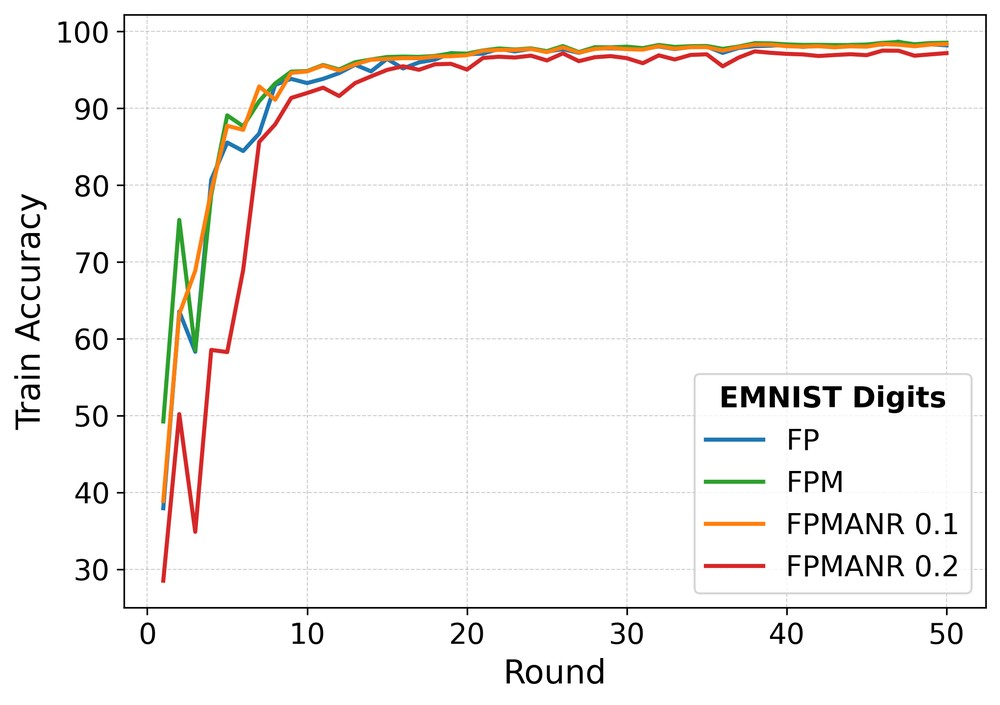
\includegraphics[width=0.235\textwidth]{figures/image5.jpg} & 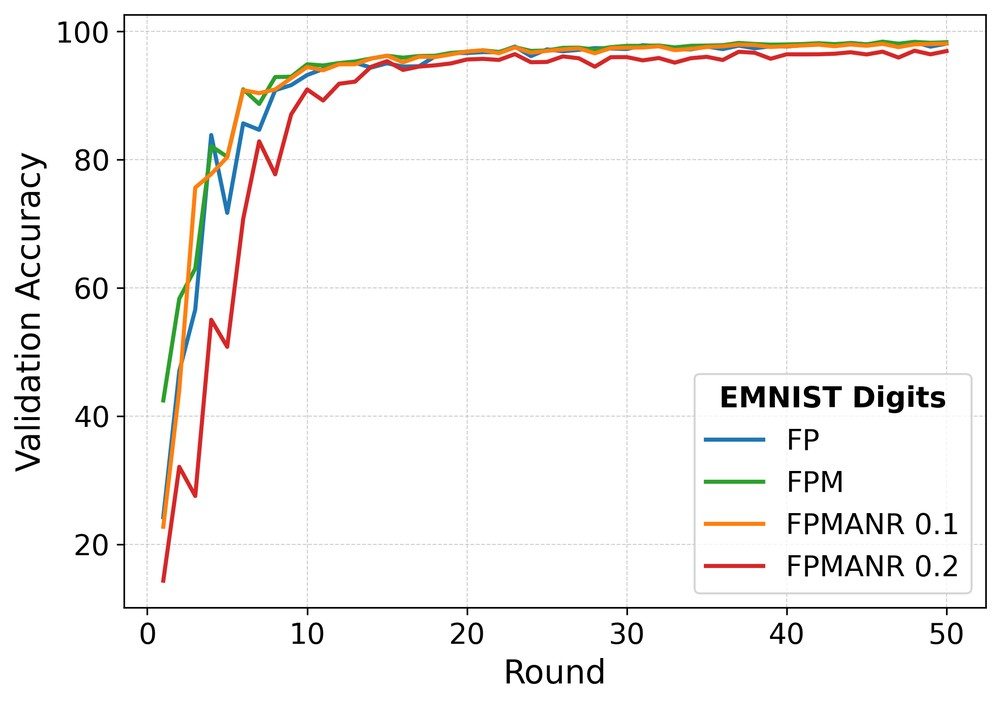
\includegraphics[width=0.235\textwidth]{figures/image6.jpg} & 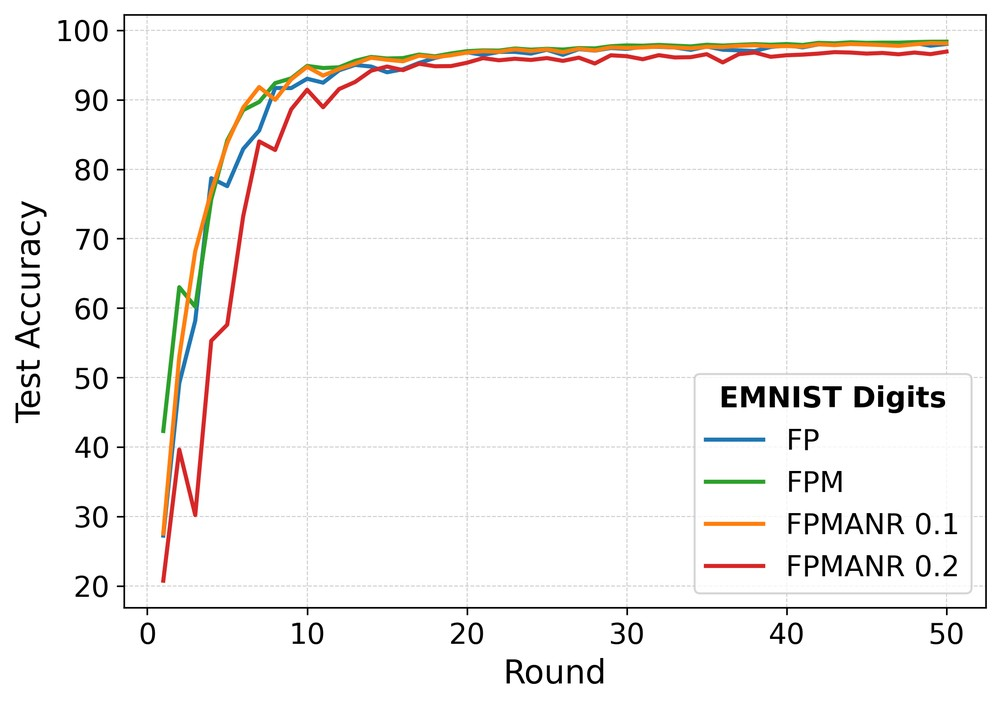
\includegraphics[width=0.235\textwidth]{figures/image7.jpg} & 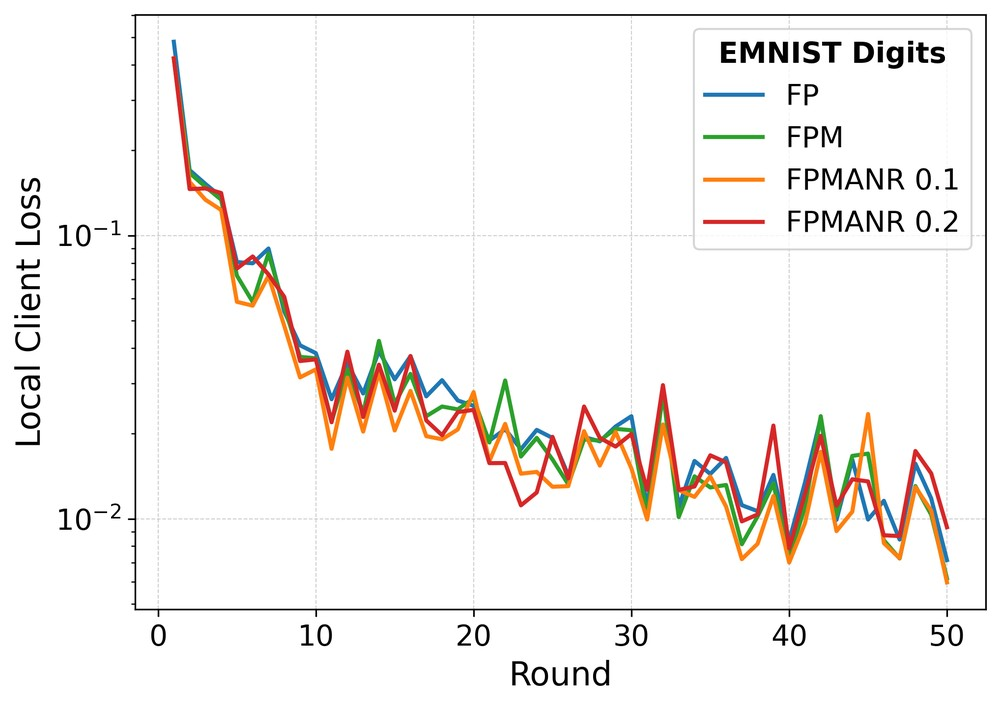
\includegraphics[width=0.235\textwidth]{figures/image8.jpg} \\
(i.a) & (i.b) & (i.c) & (i.d) \\
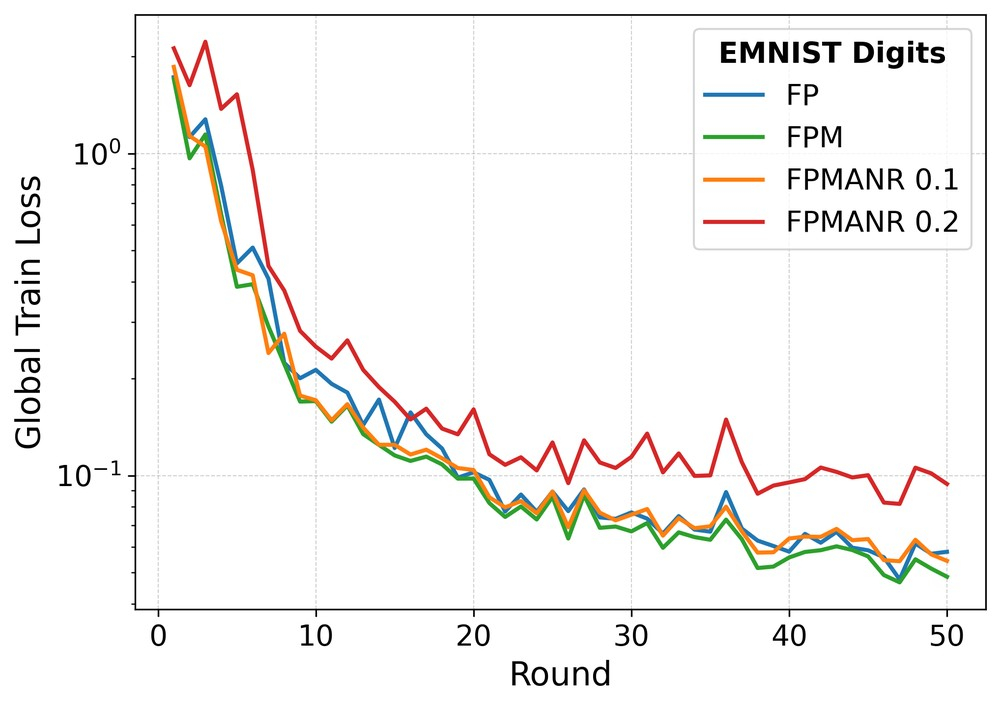
\includegraphics[width=0.235\textwidth]{figures/image9.jpg} & 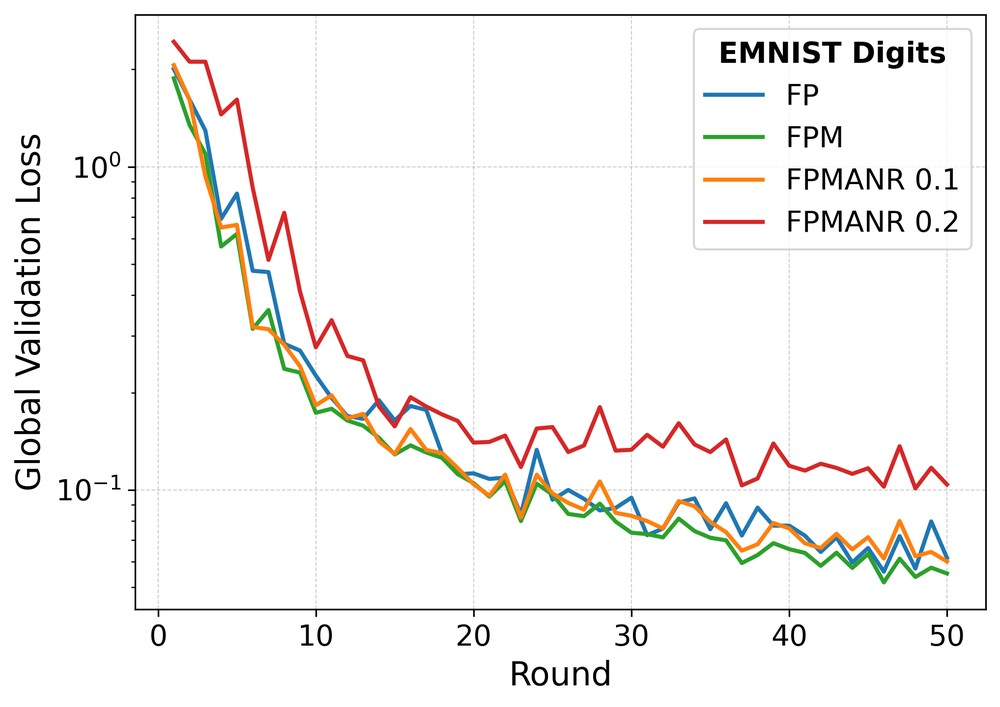
\includegraphics[width=0.235\textwidth]{figures/image10.jpg} & 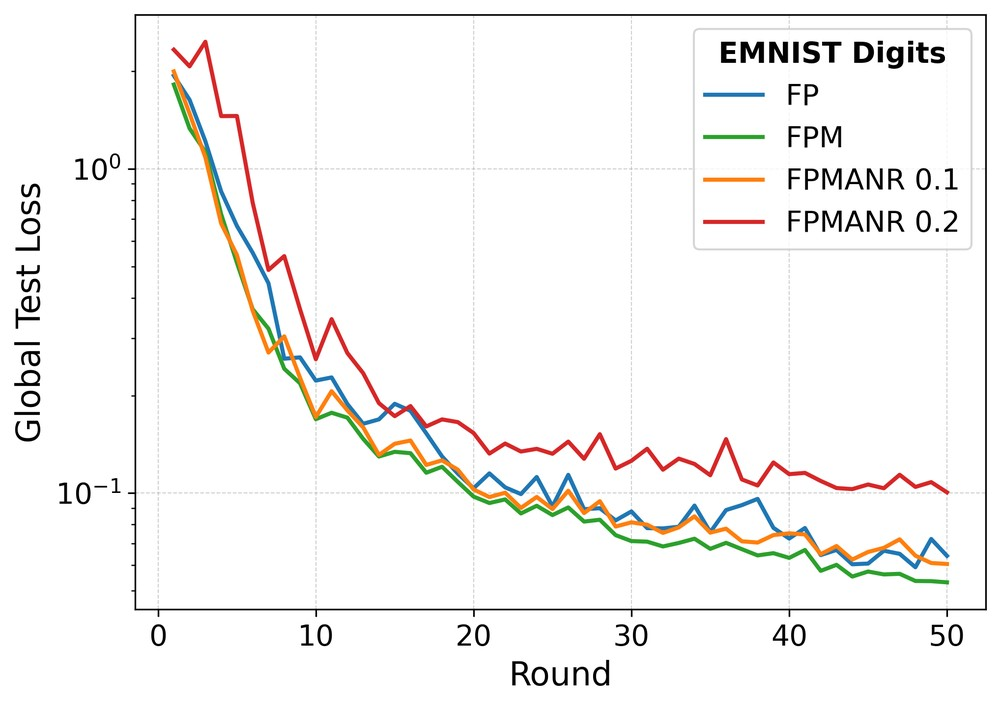
\includegraphics[width=0.235\textwidth]{figures/image11.jpg} & 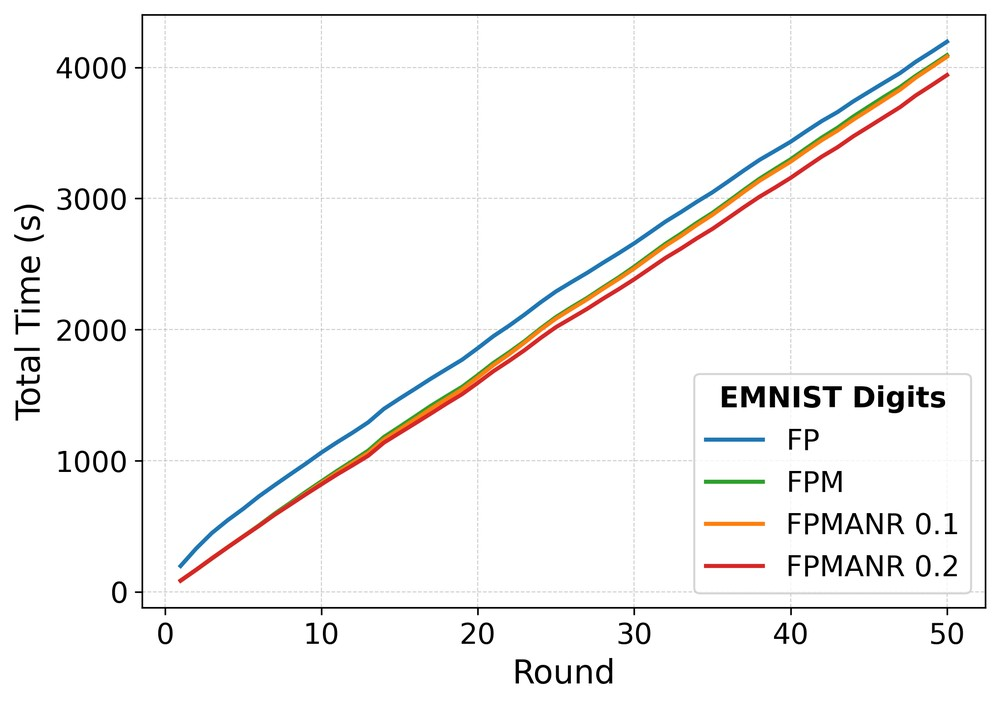
\includegraphics[width=0.235\textwidth]{figures/image12.jpg} \\
(i.e) & (i.f) & (i.g) & (i.h) \\
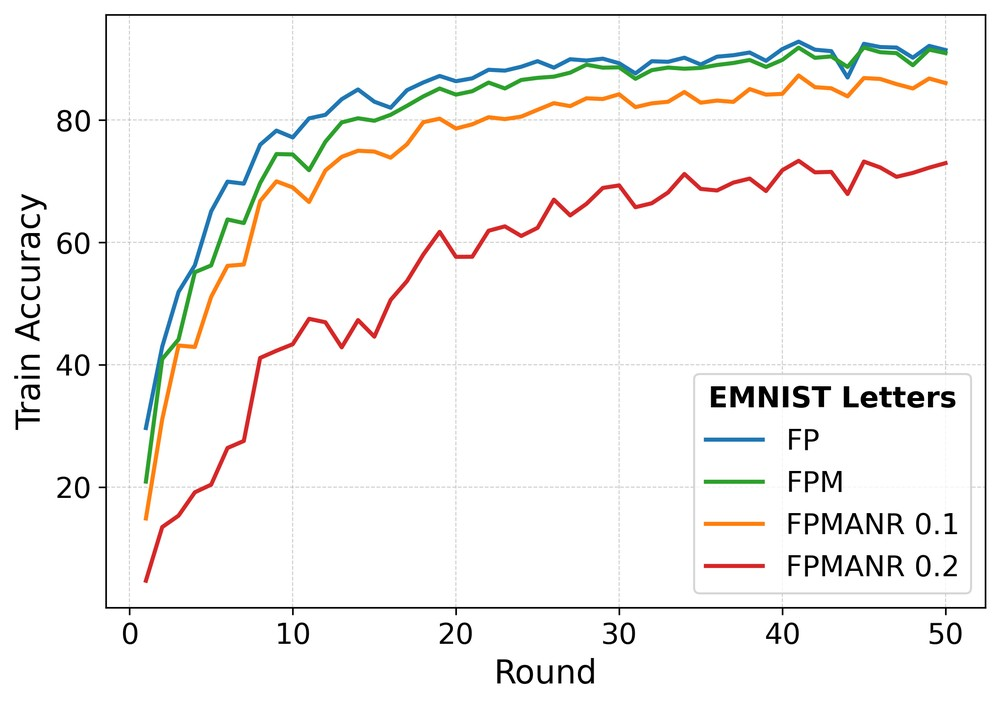
\includegraphics[width=0.235\textwidth]{figures/image13.jpg} & 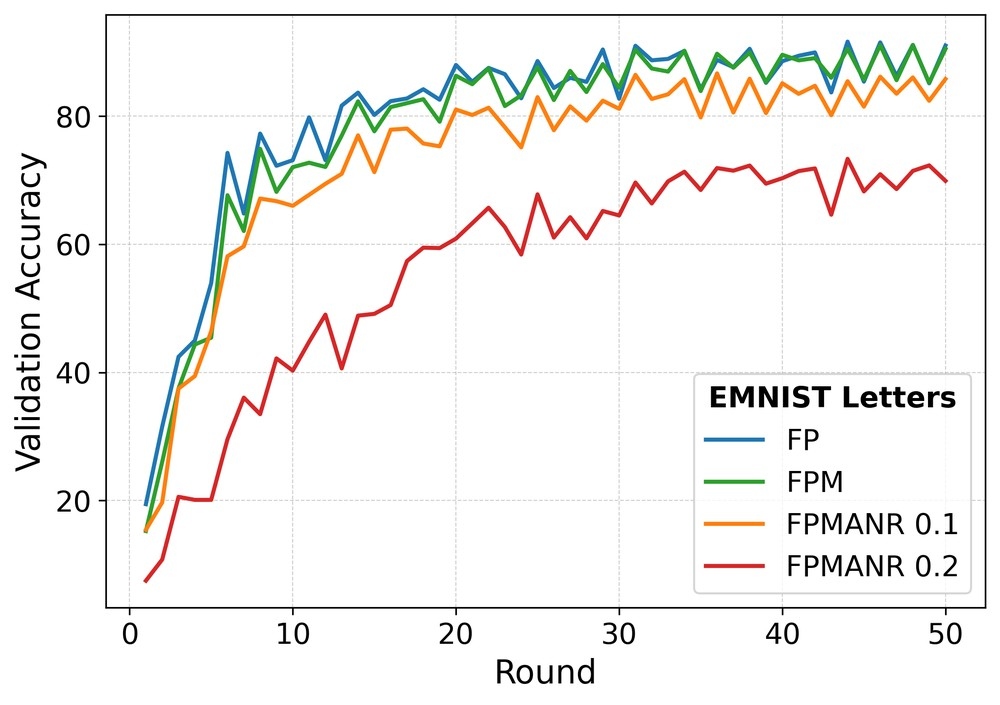
\includegraphics[width=0.235\textwidth]{figures/image14.jpg} & 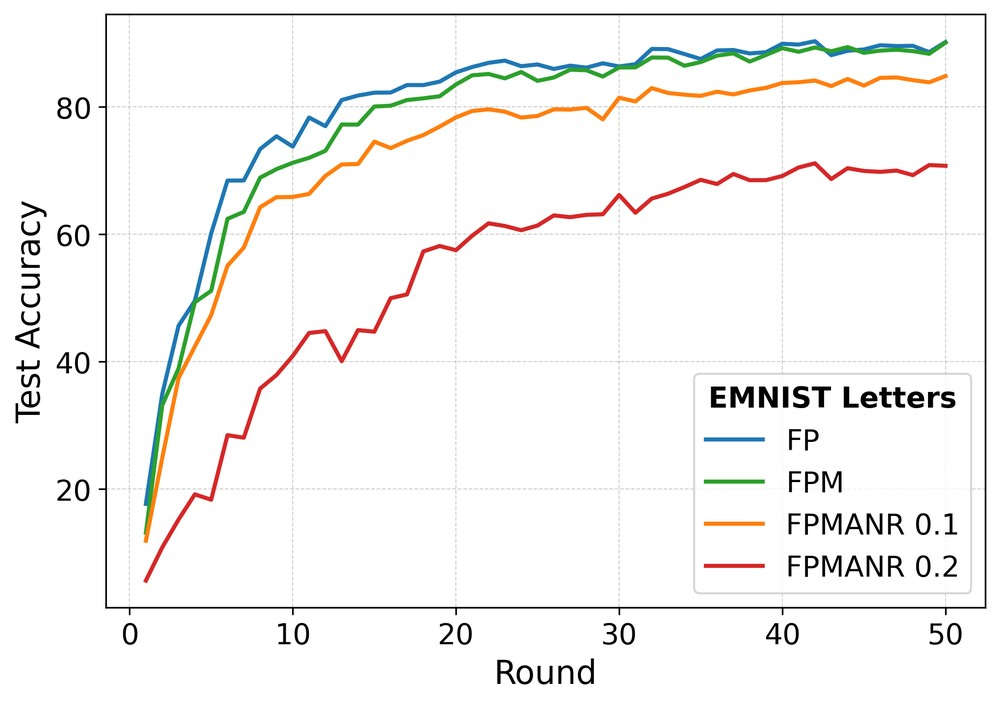
\includegraphics[width=0.235\textwidth]{figures/image15.jpg} & 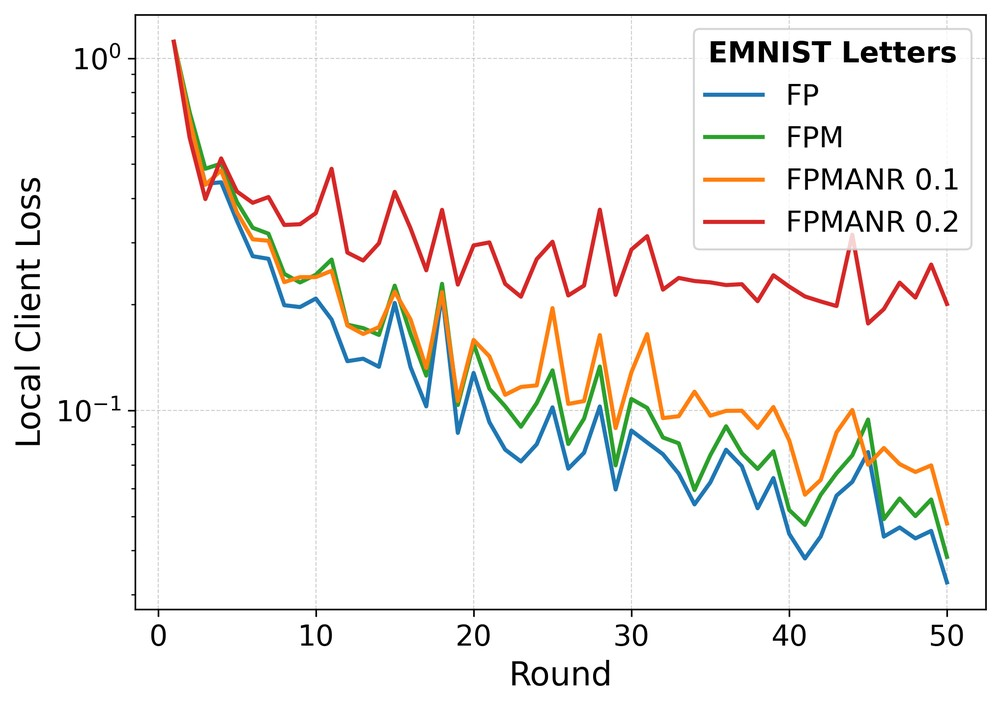
\includegraphics[width=0.235\textwidth]{figures/image16.jpg} \\
(ii.a) & (ii.b) & (ii.c) & (ii.d) \\
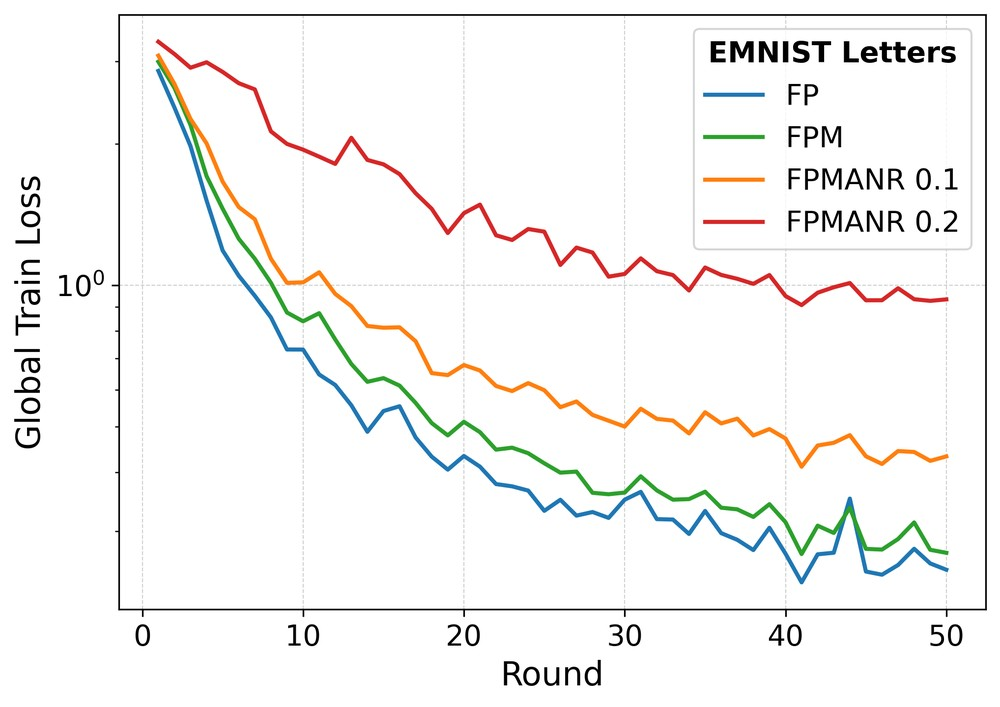
\includegraphics[width=0.235\textwidth]{figures/image17.jpg} & 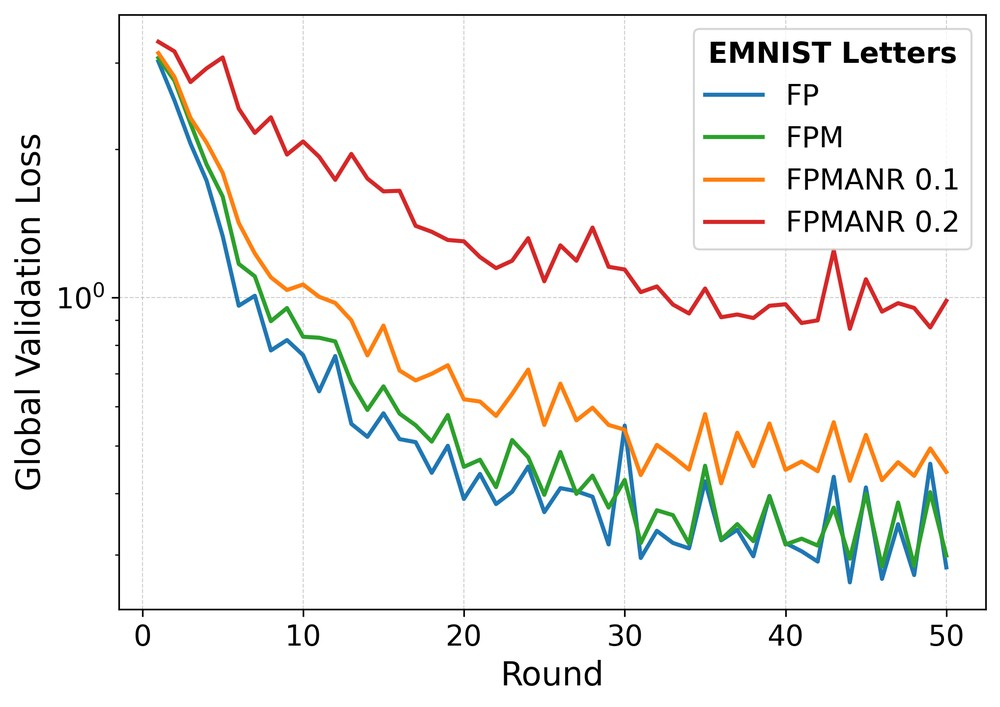
\includegraphics[width=0.235\textwidth]{figures/image18.jpg} & 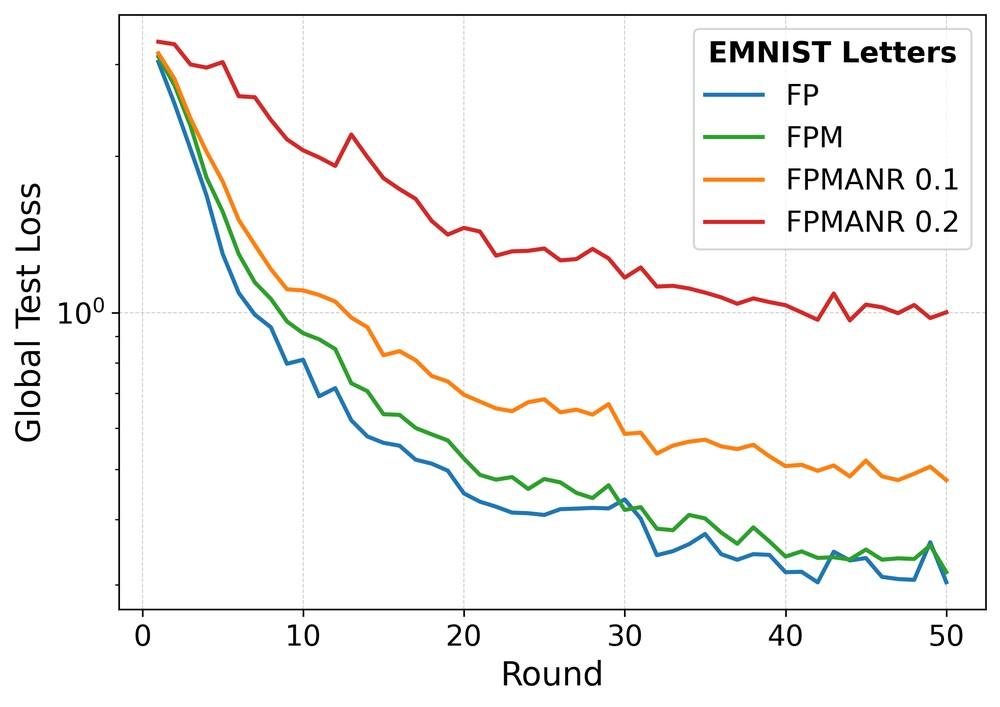
\includegraphics[width=0.235\textwidth]{figures/image19.jpg} & 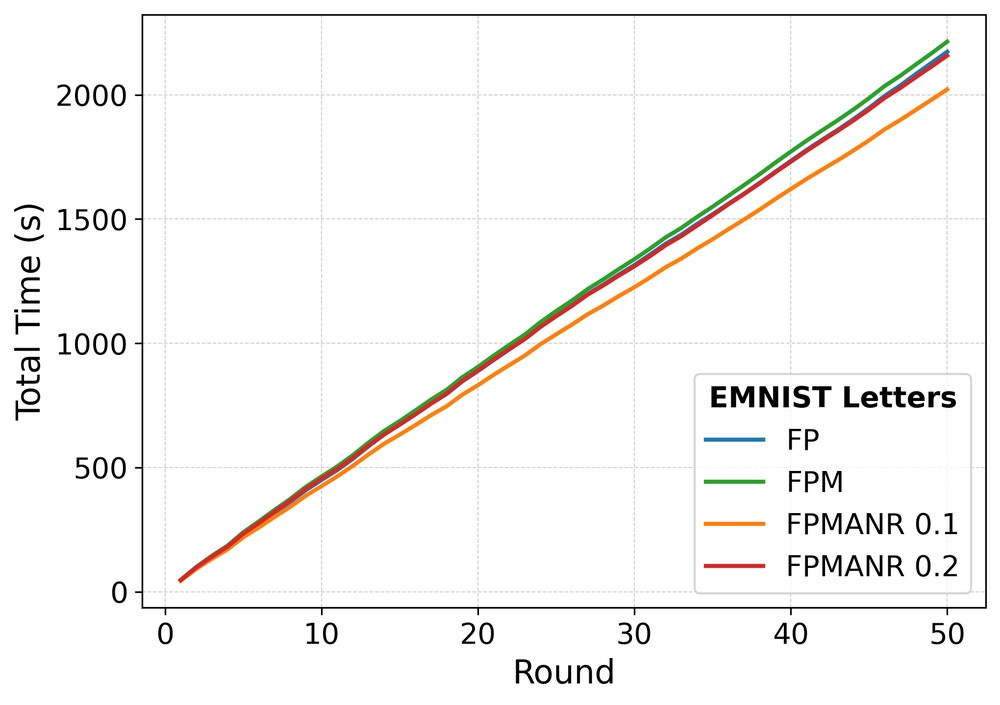
\includegraphics[width=0.235\textwidth]{figures/image20.jpg} \\
(ii.e) & (ii.f) & (ii.g) & (ii.h) \\
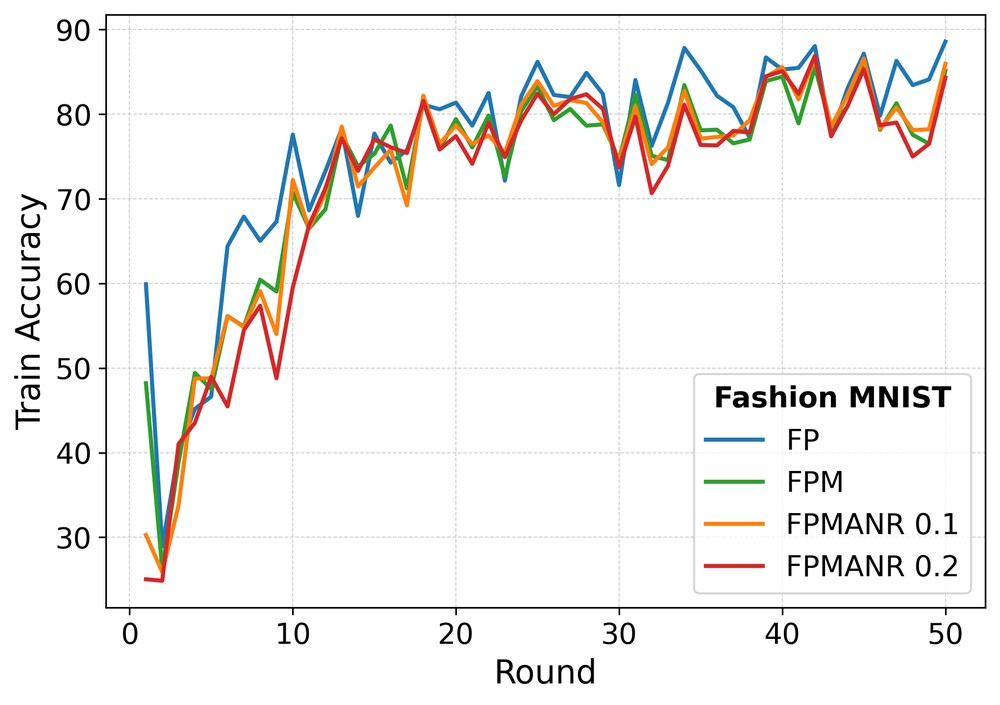
\includegraphics[width=0.235\textwidth]{figures/image21.jpg} & 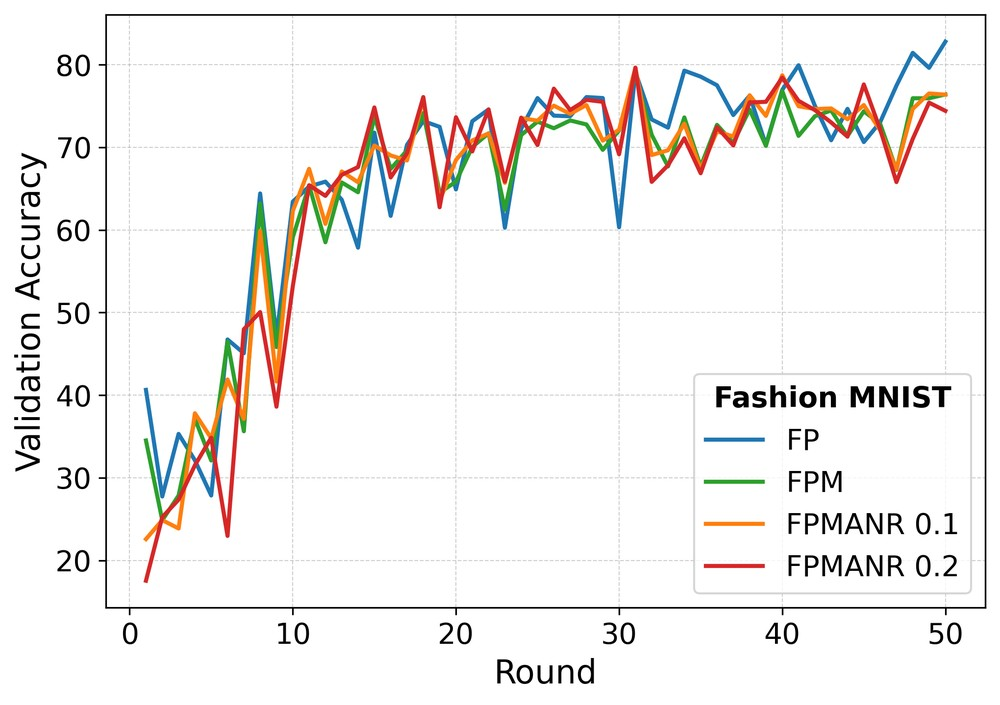
\includegraphics[width=0.235\textwidth]{figures/image22.jpg} & 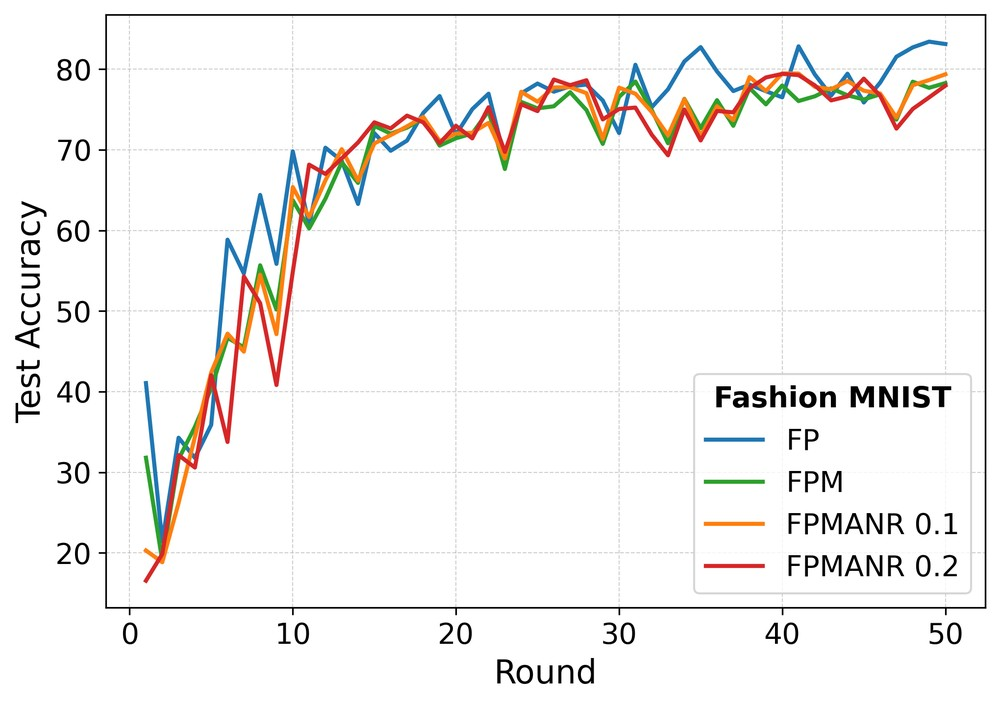
\includegraphics[width=0.235\textwidth]{figures/image23.jpg} & 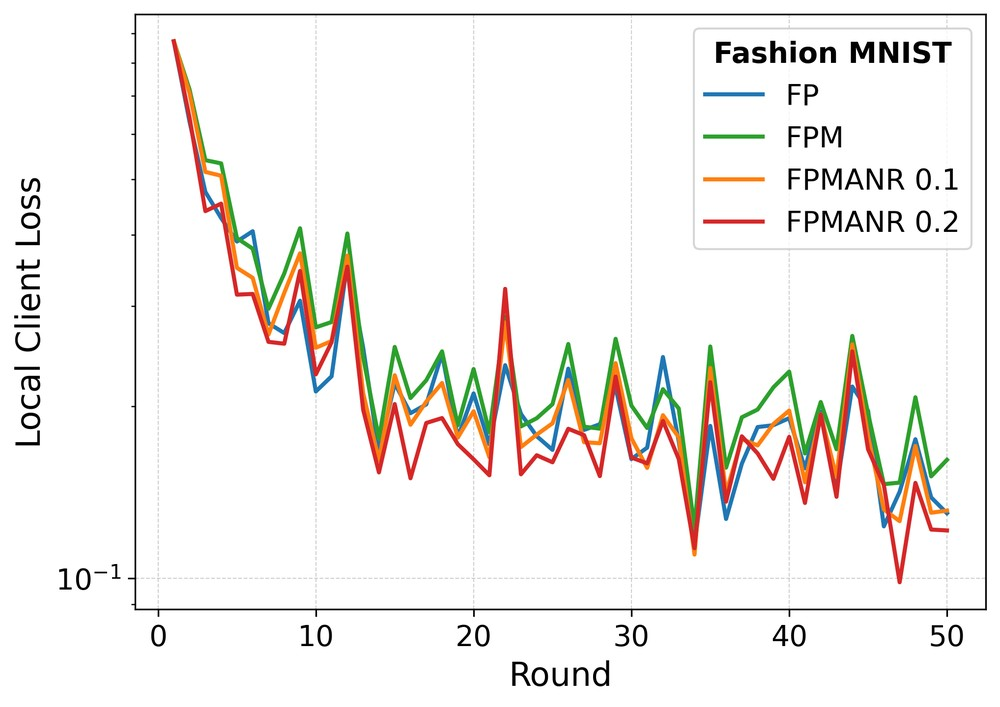
\includegraphics[width=0.235\textwidth]{figures/image24.jpg} \\
(iii.a) & (iii.b) & (iii.c) & (iii.d) \\
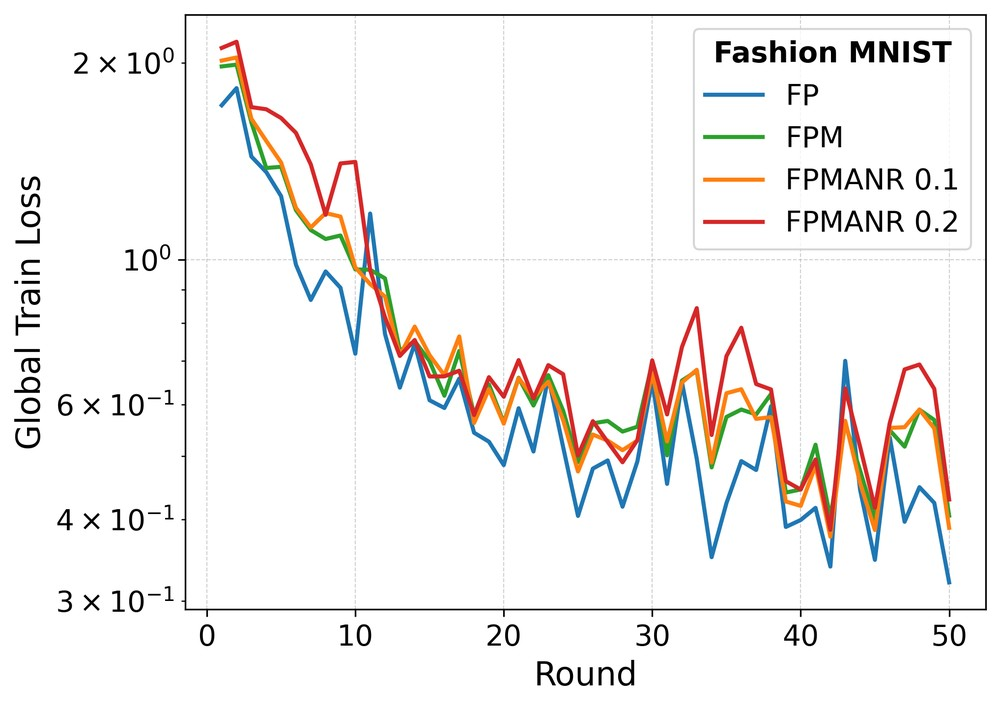
\includegraphics[width=0.235\textwidth]{figures/image25.jpg} & 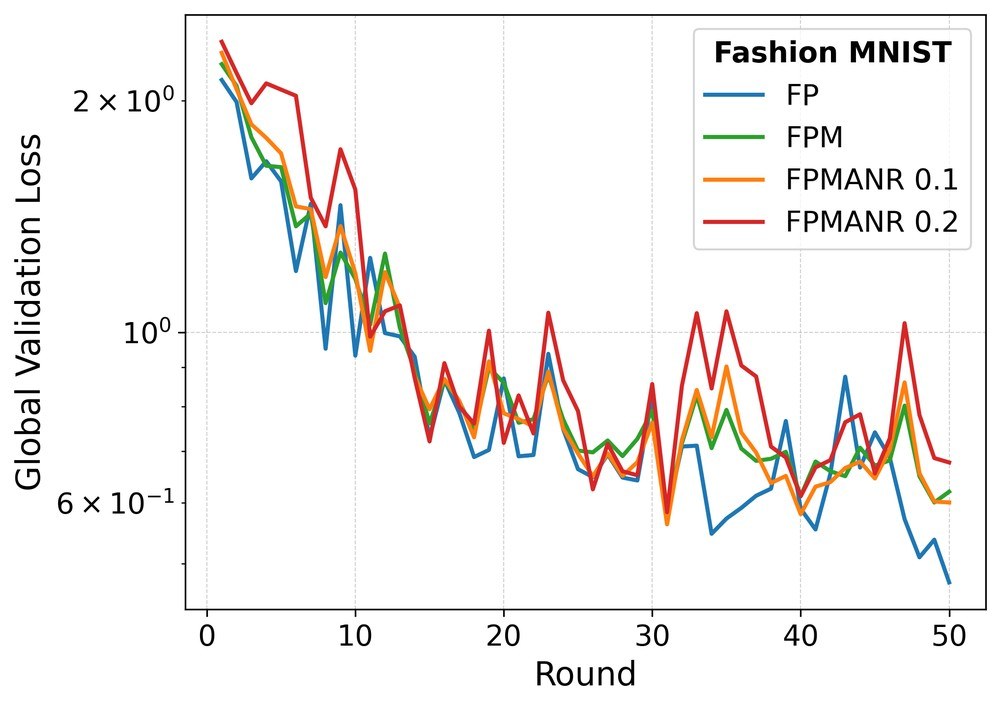
\includegraphics[width=0.235\textwidth]{figures/image26.jpg} & 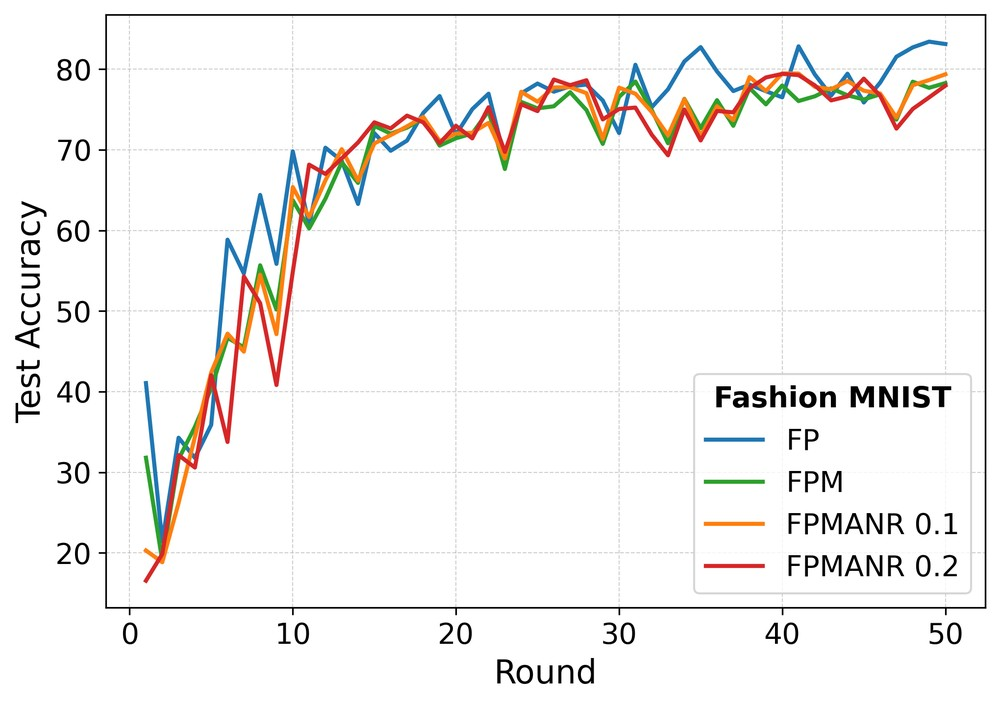
\includegraphics[width=0.235\textwidth]{figures/image23.jpg} & 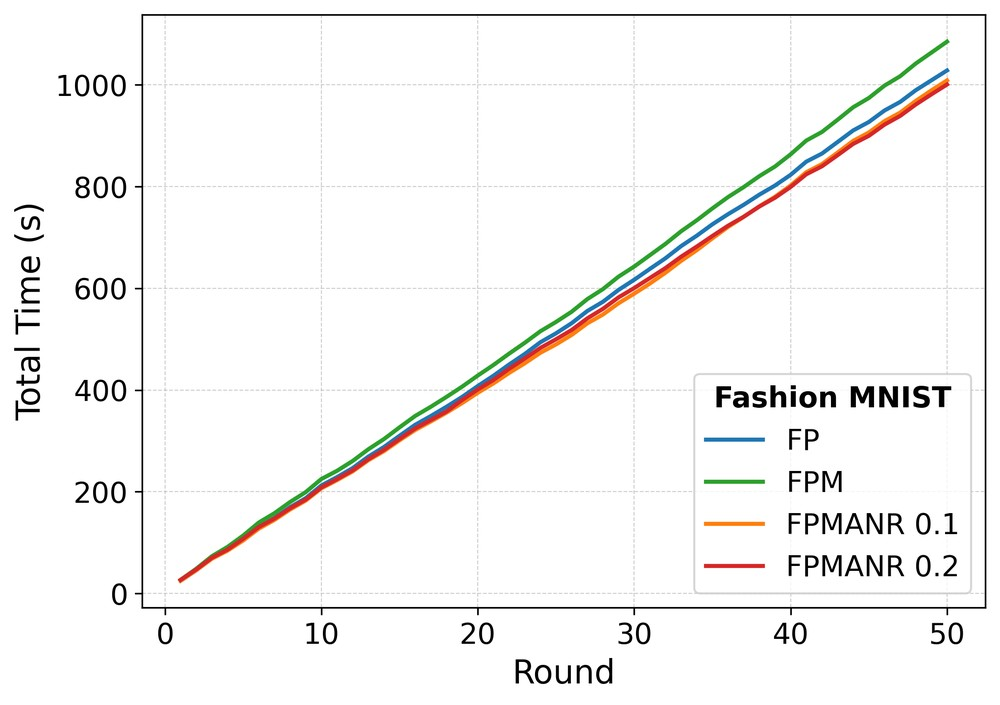
\includegraphics[width=0.235\textwidth]{figures/image27.jpg} \\
(iii.e) & (iii.f) & (iii.g) & (iii.h) \\
\end{tabular}
\caption{Accuracy, loss, and total training time over 60 rounds for FP, FPM, FPMANR 0.1, and FPMANR 0.2 on (i) EMNIST Digits, (ii) EMNIST Letters, and (iii) Fashion-MNIST.}
\label{fig:2}
\end{figure*}

Relative to FP, FPMANR 0.1 results in test accuracy reductions of 0.18\%, 5.14\%, and 6.06\% on EMNIST Digits, EMNIST Letters, and Fashion-MNIST, respectively. Increasing the ANF to 0.2 further increases the reductions to 1.35\%, 18.95\%, and 9.25\%, respectively. These results demonstrate the expected privacy--utility trade-off, where stronger adaptive noise improves privacy protection at the cost of model performance.

\subsection{Gradient Reconstruction Attack Analysis}

This section evaluates the privacy strength of the proposed framework under different attack scenarios. It analyzes gradient reconstruction attacks and MIAs to measure information leakage from shared model updates.

\xfig{fig:3} presents the visual results of gradient inversion attacks on EMNIST Digits, EMNIST Letters, and Fashion-MNIST under FP, FPM, FPMANR 0.1, and FPMANR 0.2. The first row shows the original training samples, followed by reconstructions generated using DLG, iDLG, and GradInv attacks.

\begin{figure*}
\centering
\tiny
\setlength{\tabcolsep}{2pt}
\renewcommand{\arraystretch}{1.1}
\textbf{\small EMNIST Digits}\\[1pt]
\begin{minipage}[t]{0.49\textwidth}\centering
\begin{tabular}{@{}l l c@{}}
 & Original & 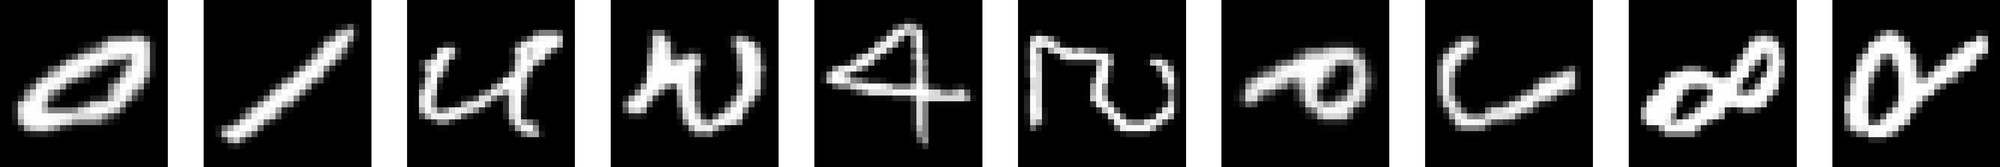
\includegraphics[width=0.40\textwidth]{figures/image28.jpg} \\
\multirow{3}{*}{\rotatebox{90}{FP}} & DLG & 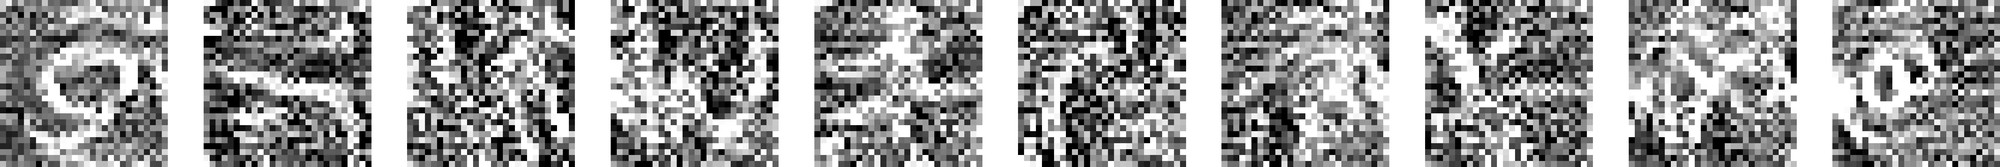
\includegraphics[width=0.40\textwidth]{figures/image29.jpg} \\
 & iDLG & 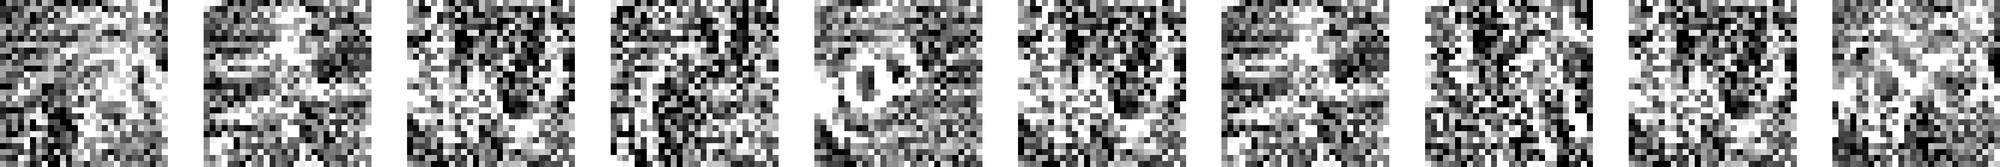
\includegraphics[width=0.40\textwidth]{figures/image30.jpg} \\
 & GradInv & 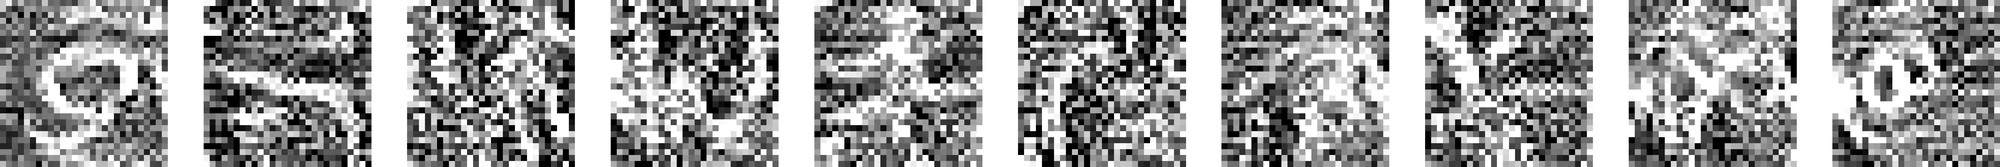
\includegraphics[width=0.40\textwidth]{figures/image31.jpg} \\
\multirow{3}{*}{\rotatebox{90}{FPM}} & DLG & 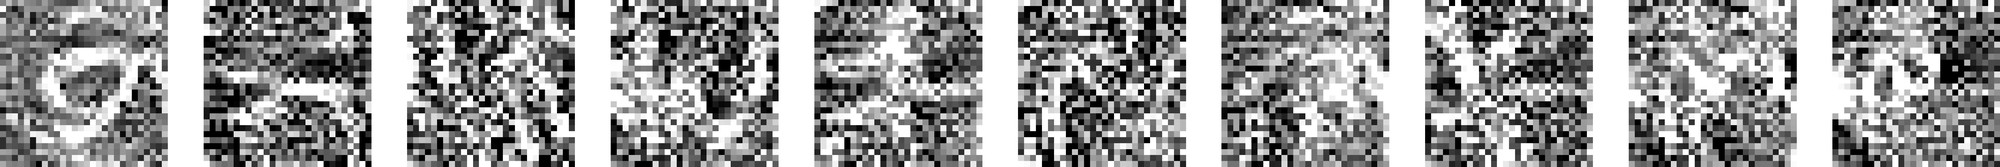
\includegraphics[width=0.40\textwidth]{figures/image32.jpg} \\
 & iDLG & 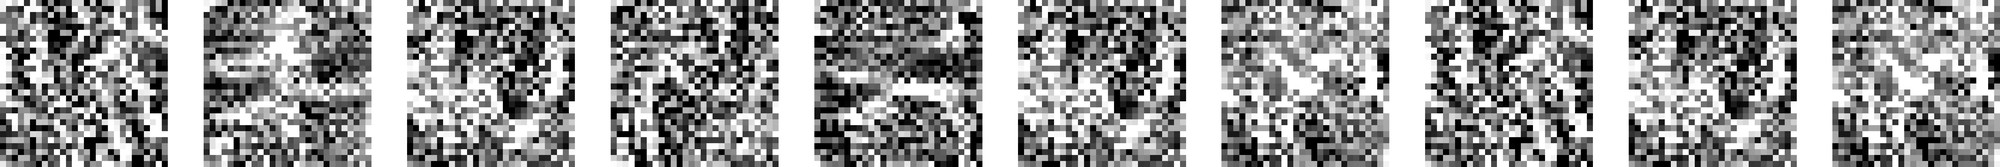
\includegraphics[width=0.40\textwidth]{figures/image33.jpg} \\
 & GradInv & 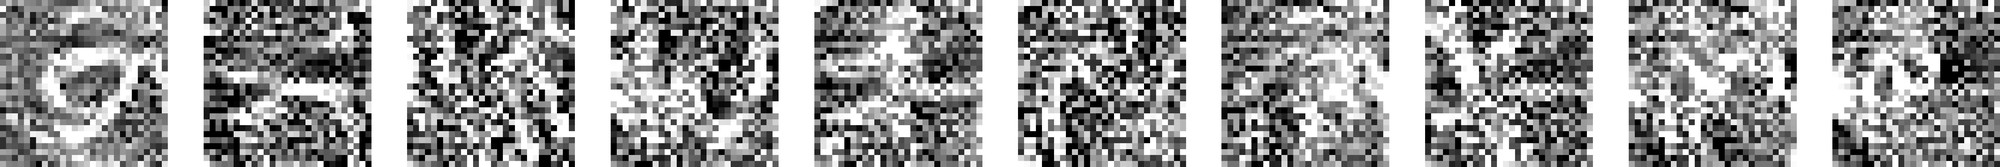
\includegraphics[width=0.40\textwidth]{figures/image34.jpg} \\
\end{tabular}
\end{minipage}
\hfill
\begin{minipage}[t]{0.49\textwidth}\centering
\begin{tabular}{@{}l l c@{}}
\multirow{3}{*}{\rotatebox{90}{\shortstack{FPMANR\\0.1}}} & DLG & 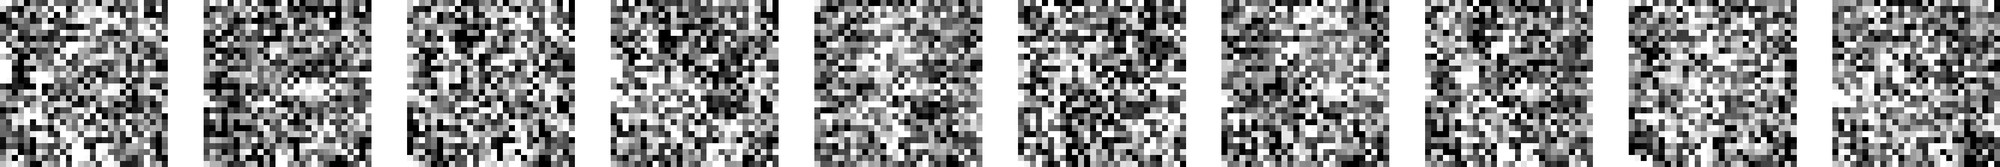
\includegraphics[width=0.40\textwidth]{figures/image35.jpg} \\
 & iDLG & 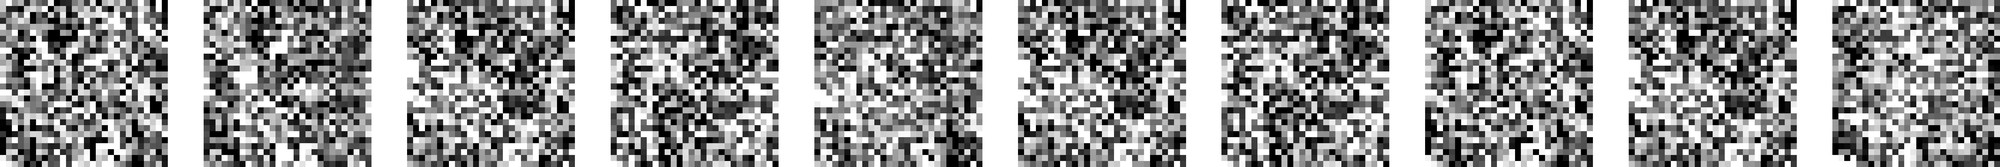
\includegraphics[width=0.40\textwidth]{figures/image36.jpg} \\
 & GradInv & 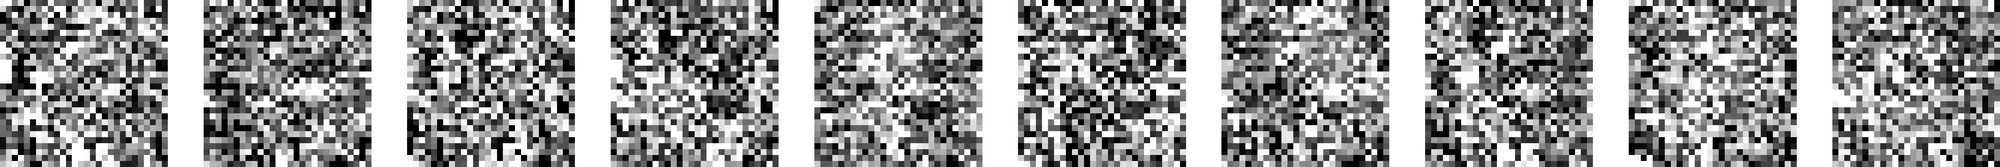
\includegraphics[width=0.40\textwidth]{figures/image37.jpg} \\
\multirow{3}{*}{\rotatebox{90}{\shortstack{FPMANR\\0.2}}} & DLG & 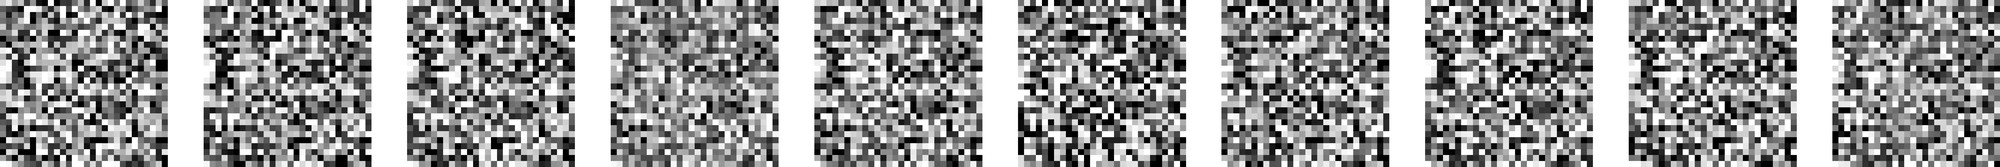
\includegraphics[width=0.40\textwidth]{figures/image38.jpg} \\
 & iDLG & 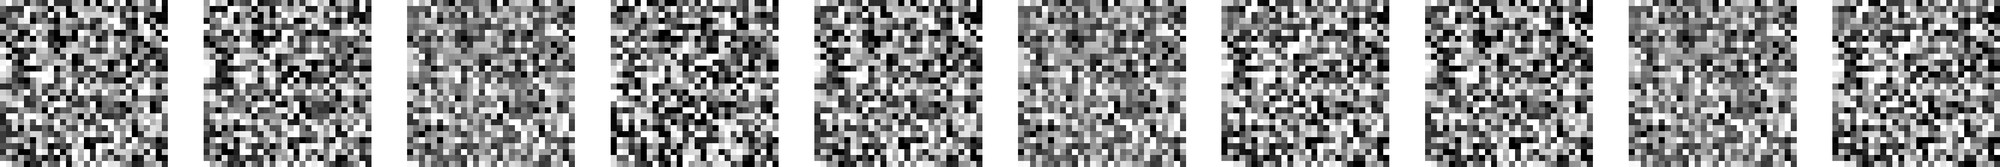
\includegraphics[width=0.40\textwidth]{figures/image39.jpg} \\
 & GradInv & 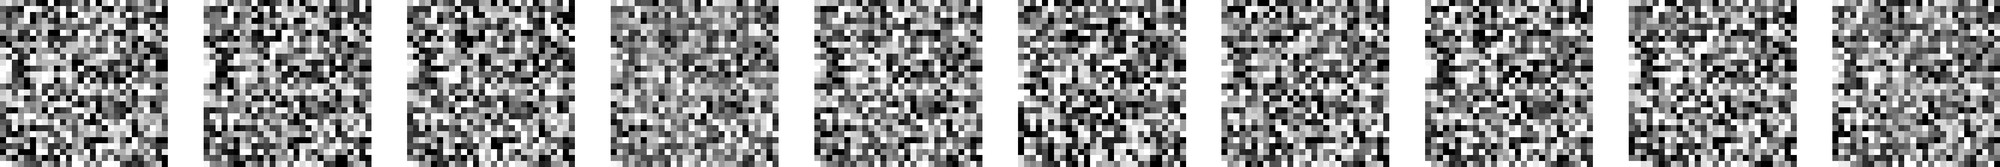
\includegraphics[width=0.40\textwidth]{figures/image40.jpg} \\
\end{tabular}
\end{minipage}
\\[6pt]
\textbf{\small EMNIST Letters}\\[1pt]
\begin{minipage}[t]{0.49\textwidth}\centering
\begin{tabular}{@{}l l c@{}}
 & Original & 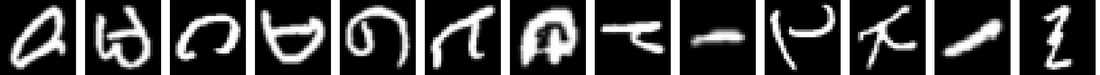
\includegraphics[width=0.40\textwidth]{figures/image41_a.jpg} \\
 & & 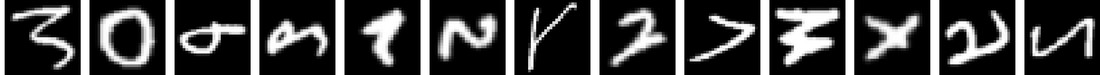
\includegraphics[width=0.40\textwidth]{figures/image41_b.jpg} \\
\multirow{6}{*}{\rotatebox{90}{FP}} & DLG & 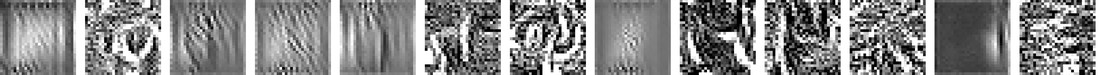
\includegraphics[width=0.40\textwidth]{figures/image42_a.jpg} \\
 & & 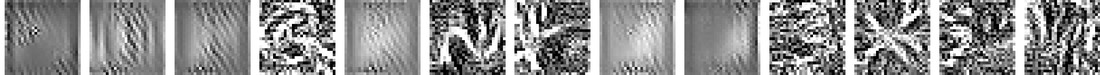
\includegraphics[width=0.40\textwidth]{figures/image42_b.jpg} \\
 & iDLG & 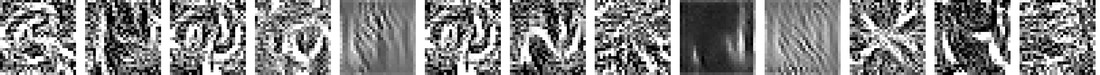
\includegraphics[width=0.40\textwidth]{figures/image43_a.jpg} \\
 & & 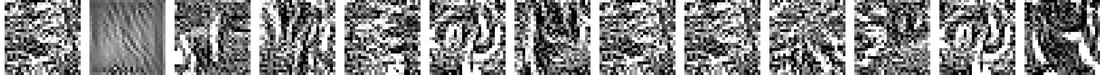
\includegraphics[width=0.40\textwidth]{figures/image43_b.jpg} \\
 & GradInv & 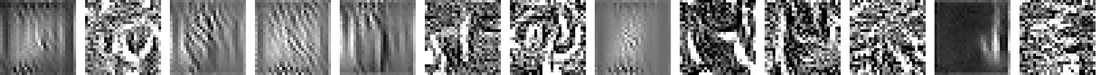
\includegraphics[width=0.40\textwidth]{figures/image44_a.jpg} \\
 & & 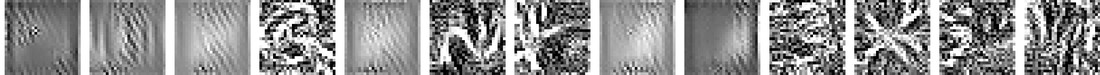
\includegraphics[width=0.40\textwidth]{figures/image44_b.jpg} \\
\multirow{6}{*}{\rotatebox{90}{FPM}} & DLG & 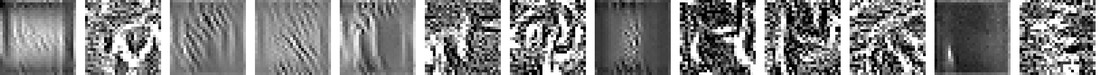
\includegraphics[width=0.40\textwidth]{figures/image45_a.jpg} \\
 & & 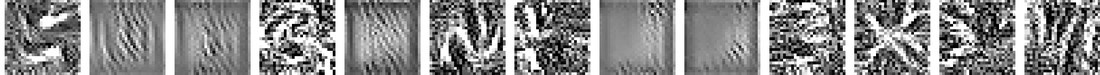
\includegraphics[width=0.40\textwidth]{figures/image45_b.jpg} \\
 & iDLG & 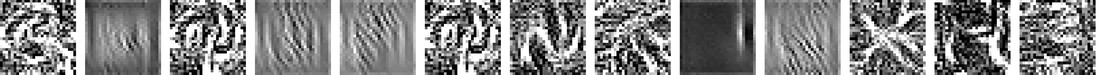
\includegraphics[width=0.40\textwidth]{figures/image46_a.jpg} \\
 & & 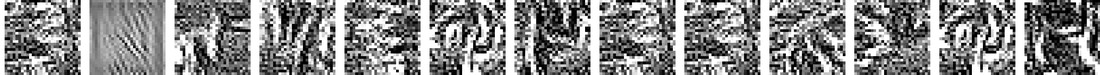
\includegraphics[width=0.40\textwidth]{figures/image46_b.jpg} \\
 & GradInv & 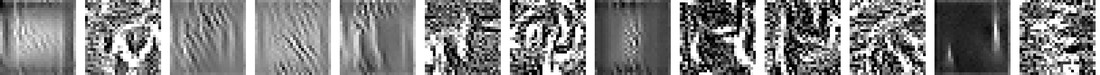
\includegraphics[width=0.40\textwidth]{figures/image47_a.jpg} \\
 & & 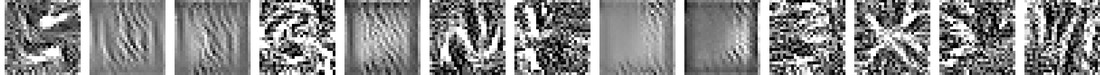
\includegraphics[width=0.40\textwidth]{figures/image47_b.jpg} \\
\end{tabular}
\end{minipage}
\hfill
\begin{minipage}[t]{0.49\textwidth}\centering
\begin{tabular}{@{}l l c@{}}
\multirow{6}{*}{\rotatebox{90}{\shortstack{FPMANR\\0.1}}} & DLG & 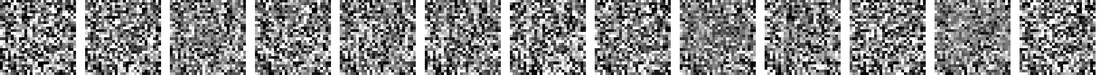
\includegraphics[width=0.40\textwidth]{figures/image48_a.jpg} \\
 & & 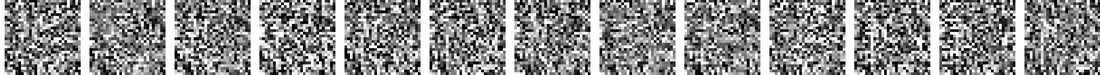
\includegraphics[width=0.40\textwidth]{figures/image48_b.jpg} \\
 & iDLG & 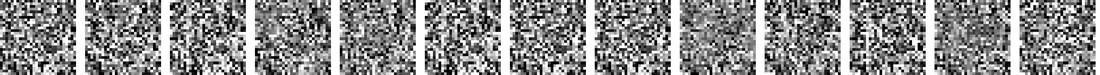
\includegraphics[width=0.40\textwidth]{figures/image49_a.jpg} \\
 & & 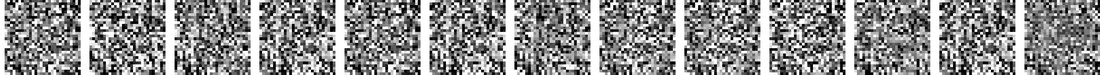
\includegraphics[width=0.40\textwidth]{figures/image49_b.jpg} \\
 & GradInv & 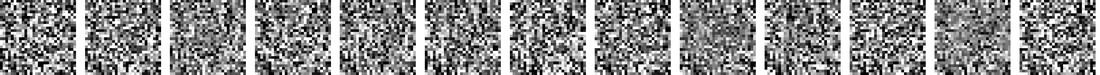
\includegraphics[width=0.40\textwidth]{figures/image50_a.jpg} \\
 & & 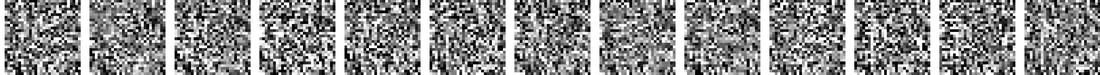
\includegraphics[width=0.40\textwidth]{figures/image50_b.jpg} \\
\multirow{6}{*}{\rotatebox{90}{\shortstack{FPMANR\\0.2}}} & DLG & 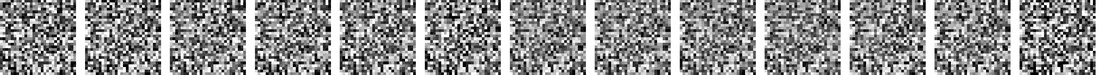
\includegraphics[width=0.40\textwidth]{figures/image51_a.jpg} \\
 & & 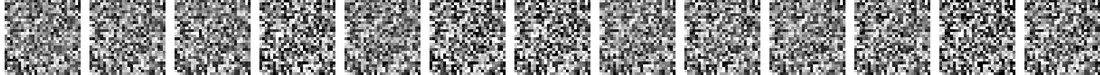
\includegraphics[width=0.40\textwidth]{figures/image51_b.jpg} \\
 & iDLG & 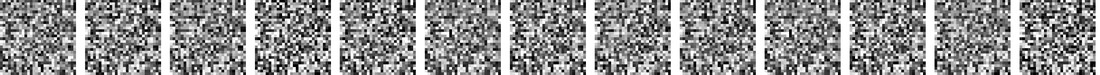
\includegraphics[width=0.40\textwidth]{figures/image52_a.jpg} \\
 & & 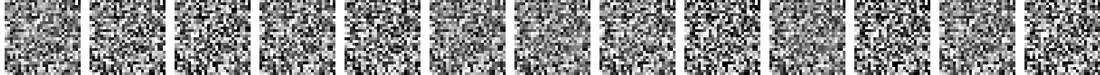
\includegraphics[width=0.40\textwidth]{figures/image52_b.jpg} \\
 & GradInv & 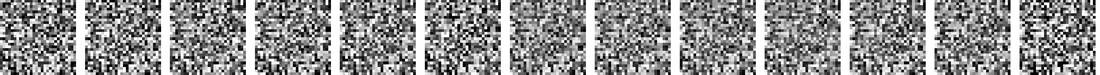
\includegraphics[width=0.40\textwidth]{figures/image53_a.jpg} \\
 & & 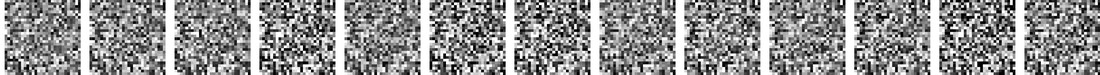
\includegraphics[width=0.40\textwidth]{figures/image53_b.jpg} \\
\end{tabular}
\end{minipage}
\\[6pt]
\textbf{\small Fashion-MNIST}\\[1pt]
\begin{minipage}[t]{0.49\textwidth}\centering
\begin{tabular}{@{}l l c@{}}
 & Original & 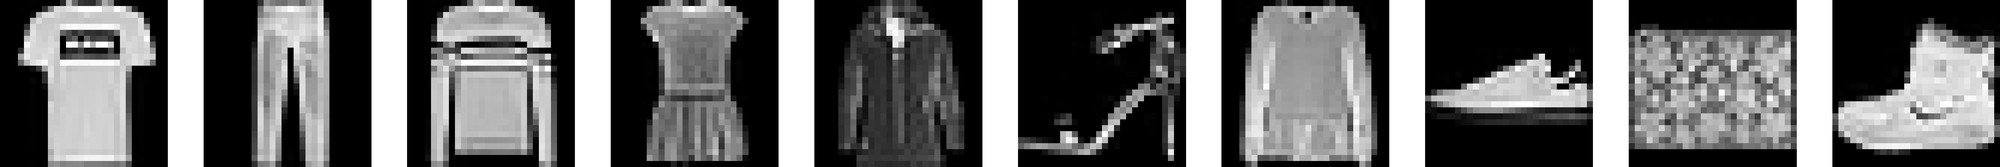
\includegraphics[width=0.40\textwidth]{figures/image54.jpg} \\
\multirow{3}{*}{\rotatebox{90}{FP}} & DLG & 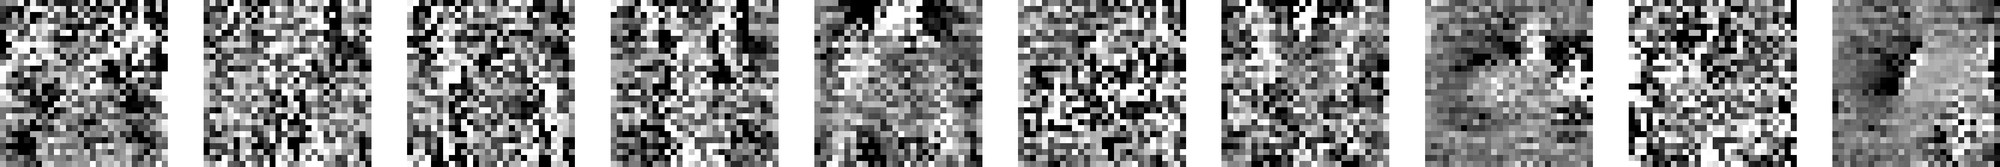
\includegraphics[width=0.40\textwidth]{figures/image55.jpg} \\
 & iDLG & 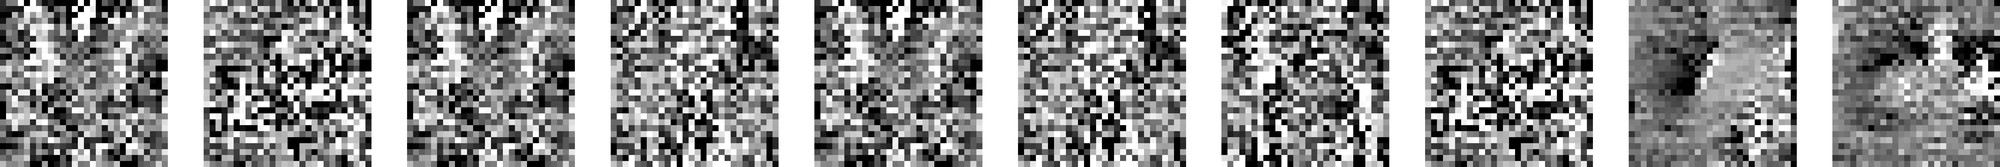
\includegraphics[width=0.40\textwidth]{figures/image56.jpg} \\
 & GradInv & 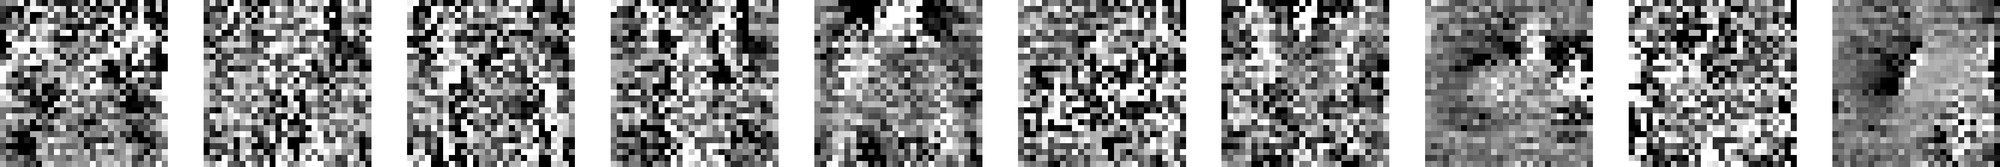
\includegraphics[width=0.40\textwidth]{figures/image57.jpg} \\
\multirow{3}{*}{\rotatebox{90}{FPM}} & DLG & 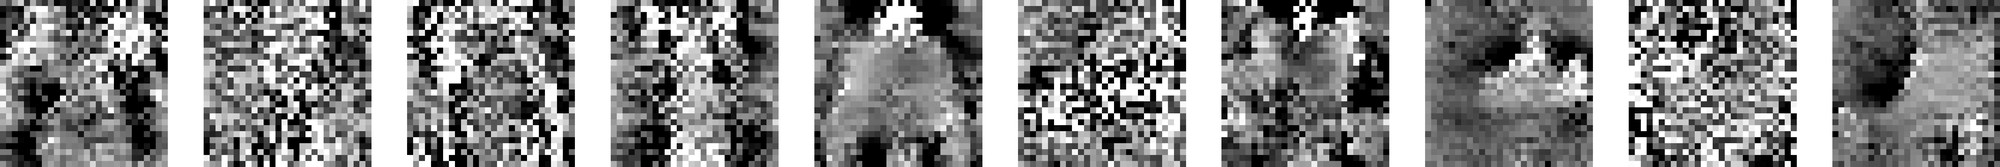
\includegraphics[width=0.40\textwidth]{figures/image58.jpg} \\
 & iDLG & 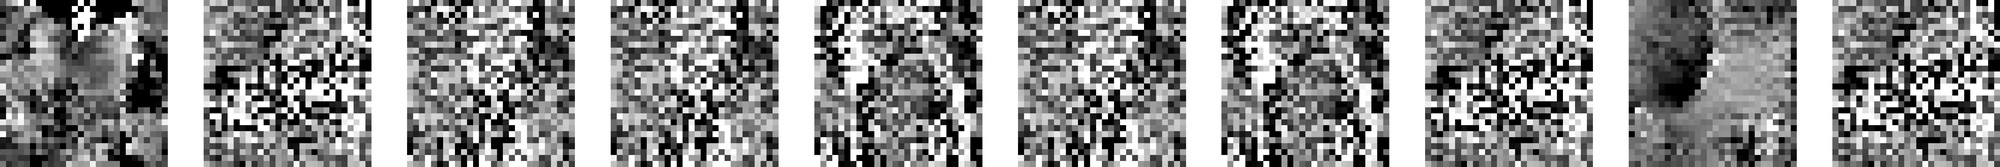
\includegraphics[width=0.40\textwidth]{figures/image59.jpg} \\
 & GradInv & 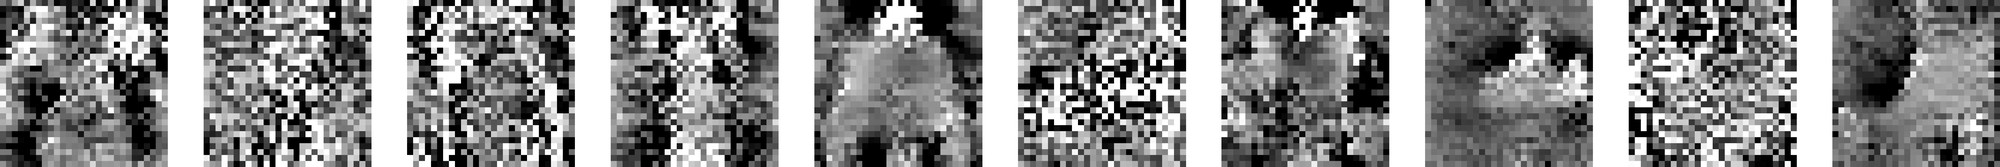
\includegraphics[width=0.40\textwidth]{figures/image60.jpg} \\
\end{tabular}
\end{minipage}
\hfill
\begin{minipage}[t]{0.49\textwidth}\centering
\begin{tabular}{@{}l l c@{}}
\multirow{3}{*}{\rotatebox{90}{\shortstack{FPMANR\\0.1}}} & DLG & 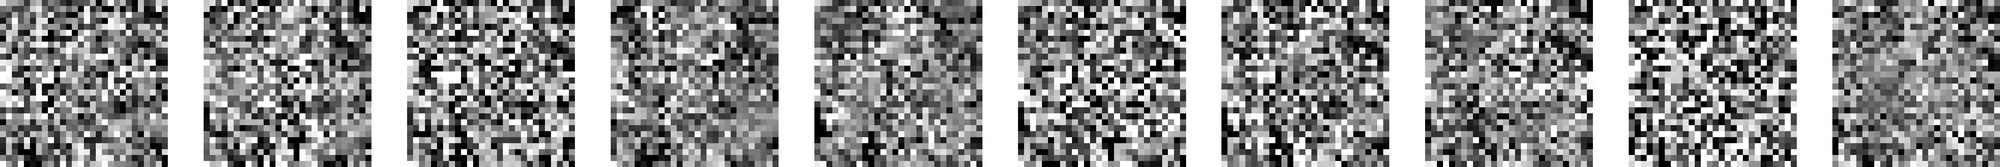
\includegraphics[width=0.40\textwidth]{figures/image61.jpg} \\
 & iDLG & 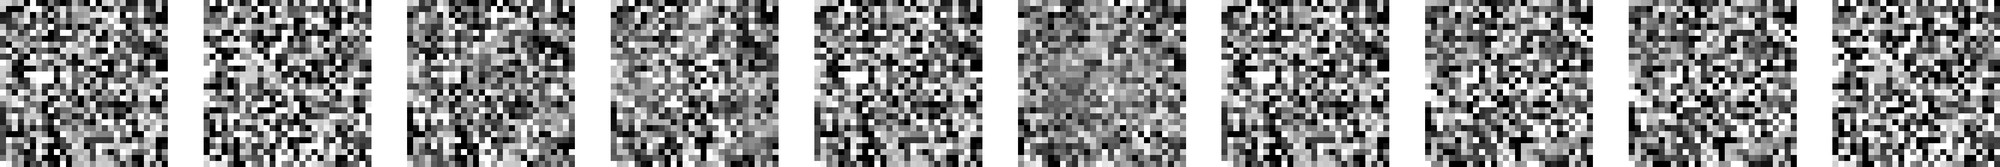
\includegraphics[width=0.40\textwidth]{figures/image62.jpg} \\
 & GradInv & 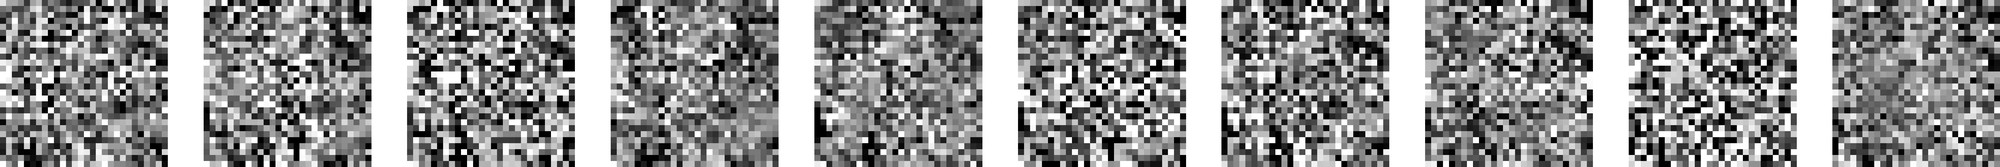
\includegraphics[width=0.40\textwidth]{figures/image63.jpg} \\
\multirow{3}{*}{\rotatebox{90}{\shortstack{FPMANR\\0.2}}} & DLG & 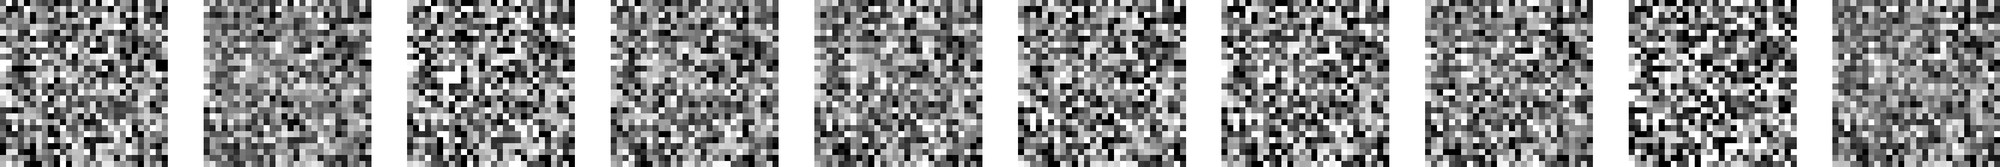
\includegraphics[width=0.40\textwidth]{figures/image64.jpg} \\
 & iDLG & 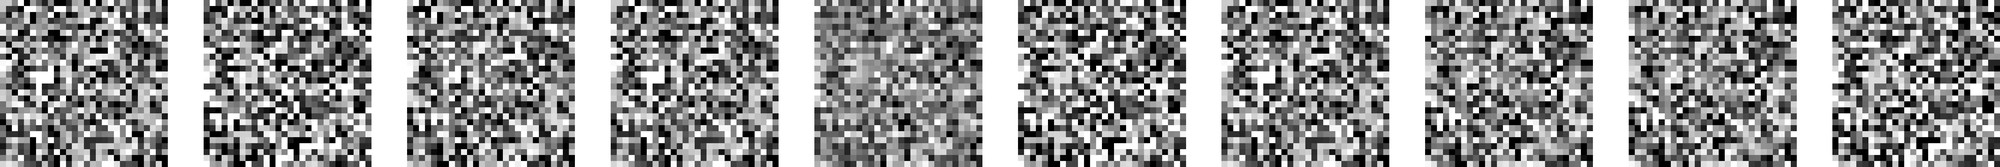
\includegraphics[width=0.40\textwidth]{figures/image65.jpg} \\
 & GradInv & 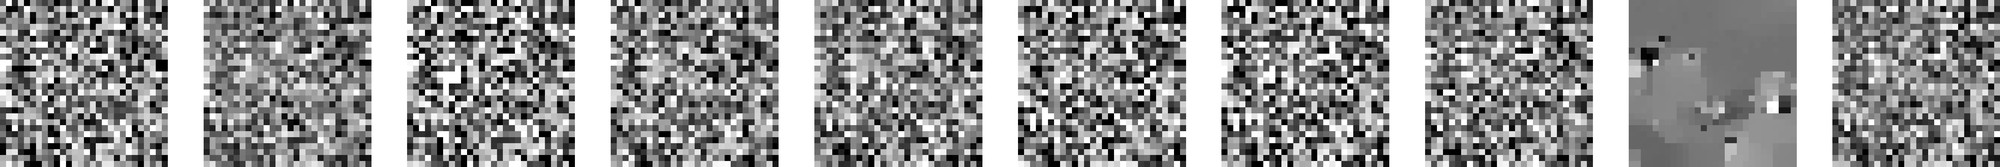
\includegraphics[width=0.40\textwidth]{figures/image66.jpg} \\
\end{tabular}
\end{minipage}
\\[6pt]
\caption{Gradient reconstruction results on EMNIST Digits, EMNIST Letters, and Fashion-MNIST under FP, FPM, FPMANR 0.1, and FPMANR 0.2.}
\label{fig:3}
\end{figure*}

Under FP, all three attacks are able to recover recognizable image structures from the shared client updates, with GradInv producing the clearest reconstructions due to its stronger optimization and regularization mechanisms. The recovered digits, letters, and clothing shapes indicate that substantial input information remains embedded in the transmitted updates.

When pairwise masking is introduced in FPM, the reconstruction quality decreases noticeably because each client update is perturbed by random pairwise masks prior to aggregation. Although the masks cancel during global aggregation, the individual shared updates become less consistent for inversion-based optimization, thereby reducing reconstruction fidelity. Nevertheless, partial low-level structures and coarse semantic patterns remain observable in some samples.

After adaptive noise is incorporated in FPMANR 0.1 and FPMANR 0.2, the reconstructed images become increasingly distorted and visually unrecognizable. Since the injected noise is scaled according to the magnitude of each layer update, the perturbed updates differ further from the original shared updates, making gradient matching substantially more difficult for the attacker. As the ANF increases, the signal-to-noise ratio of the shared updates decreases further, leading to progressively weaker recoverable information. FPMANR 0.1 already provides a clear reduction in reconstruction quality compared to FPM, while FPMANR 0.2 further strengthens this effect by introducing higher perturbation, resulting in the most severe distortion. Overall, both FPMANR settings consistently outperform the other configurations in terms of resistance to reconstruction attacks across all datasets and attack methods.

\xtab{tab:1} quantitatively evaluates reconstruction quality using MSE, PSNR, SSIM, LPIPS, and ASR. Higher MSE and LPIPS indicate larger pixel-level and perceptual differences from the original images, while lower PSNR and SSIM indicate weaker visual and structural similarity. ASR is defined as the percentage of reconstructed samples satisfying SSIM $\geq$ 0.1 or PSNR $\geq$ 10. Lower ASR means fewer successfully recognizable reconstructions.

Across all datasets, FP and FPM generally produce lower MSE and LPIPS together with higher PSNR, SSIM, and ASR, showing that substantial information can still be recovered from the shared updates. In some cases, FPM shows slightly higher ASR than FP because pairwise masking perturbs the updates without destroying the underlying gradient structure, and small optimization variations can occasionally make certain reconstructed samples appear more recognizable even when the overall distortion metrics remain similar.

\begin{table*}
\centering
\scriptsize
\caption{Quantitative evaluation of gradient reconstruction attacks under FP, FPM, FPMANR 0.1, and FPMANR 0.2 on EMNIST Digits, EMNIST Letters, and Fashion-MNIST using DLG, iDLG, and GradInv}
\label{tab:1}
\begin{tabular}{l l l c c c c c}
\toprule
\textbf{Dataset} & \textbf{Model} & \textbf{Attack} & \textbf{MSE $\uparrow$} & \textbf{PSNR $\downarrow$} & \textbf{SSIM $\downarrow$} & \textbf{LPIPS $\uparrow$} & \textbf{ASR $\downarrow$} \\
\midrule
\multirow{12}{*}{EMNIST Digits} & \multirow{3}{*}{FP} & DLG & 0.3151 & 5.0220 & 0.0464 & 0.6201 & 10.00\% \\
 &  & iDLG & 0.3333 & 4.7737 & 0.0195 & 0.6268 & 0.00\% \\
 &  & GradInv & 0.3149 & 5.0245 & 0.0467 & 0.6200 & 10.00\% \\
 & \multirow{3}{*}{FPM} & DLG & 0.3115 & 5.0768 & 0.0514 & 0.6350 & 10.00\% \\
 &  & iDLG & 0.3243 & 4.9051 & 0.0360 & 0.6348 & 0.00\% \\
 &  & GradInv & 0.3114 & 5.0781 & 0.0514 & 0.6349 & 10.00\% \\
 & \multirow{3}{*}{FPMANR 0.1} & DLG & 0.3201 & 4.9492 & 0.0115 & 0.6486 & 0.00\% \\
 &  & iDLG & 0.3300 & 4.8163 & 0.0167 & 0.6538 & 0.00\% \\
 &  & GradInv & 0.3200 & 4.9498 & 0.0115 & 0.6486 & 0.00\% \\
 & \multirow{3}{*}{FPMANR 0.2} & DLG & 0.3294 & 4.8242 & 0.0121 & 0.6410 & 0.00\% \\
 &  & iDLG & 0.3275 & 4.8507 & 0.0085 & 0.6410 & 0.00\% \\
 &  & GradInv & 0.3287 & 4.8332 & 0.0124 & 0.6411 & 0.00\% \\
\midrule
\multirow{12}{*}{EMNIST Letters} & \multirow{3}{*}{FP} & DLG & 0.2653 & 5.8435 & 0.0374 & 0.5661 & 7.69\% \\
 &  & iDLG & 0.2921 & 5.4771 & 0.0116 & 0.5542 & 0.00\% \\
 &  & GradInv & 0.2625 & 5.9408 & 0.0384 & 0.5617 & 3.85\% \\
 & \multirow{3}{*}{FPM} & DLG & 0.2539 & 6.0800 & 0.0395 & 0.5657 & 11.54\% \\
 &  & iDLG & 0.2831 & 5.6363 & 0.0222 & 0.5540 & 7.69\% \\
 &  & GradInv & 0.2559 & 6.0545 & 0.0407 & 0.5648 & 11.54\% \\
 & \multirow{3}{*}{FPMANR 0.1} & DLG & 0.3098 & 5.0982 & 0.0067 & 0.6529 & 0.00\% \\
 &  & iDLG & 0.3140 & 5.0388 & 0.0053 & 0.6487 & 0.00\% \\
 &  & GradInv & 0.3098 & 5.0985 & 0.0067 & 0.6529 & 0.00\% \\
 & \multirow{3}{*}{FPMANR 0.2} & DLG & 0.3147 & 5.0294 & 0.0023 & 0.6454 & 0.00\% \\
 &  & iDLG & 0.3135 & 5.0472 & 0.0010 & 0.6465 & 0.00\% \\
 &  & GradInv & 0.3146 & 5.0304 & 0.0024 & 0.6461 & 0.00\% \\
\midrule
\multirow{12}{*}{Fashion-MNIST} & \multirow{3}{*}{FP} & DLG & 0.2112 & 6.8415 & 0.0771 & 0.4809 & 40.00\% \\
 &  & iDLG & 0.2294 & 6.5660 & 0.0365 & 0.4950 & 10.00\% \\
 &  & GradInv & 0.2111 & 6.8438 & 0.0771 & 0.4808 & 40.00\% \\
 & \multirow{3}{*}{FPM} & DLG & 0.1857 & 7.4734 & 0.1078 & 0.4251 & 40.00\% \\
 &  & iDLG & 0.2365 & 6.4609 & 0.0356 & 0.4852 & 30.00\% \\
 &  & GradInv & 0.1856 & 7.4744 & 0.1078 & 0.4254 & 40.00\% \\
 & \multirow{3}{*}{FPMANR 0.1} & DLG & 0.2244 & 6.5520 & 0.0216 & 0.5102 & 0.00\% \\
 &  & iDLG & 0.2491 & 6.0995 & -0.0011 & 0.5173 & 0.00\% \\
 &  & GradInv & 0.2242 & 6.5555 & 0.0216 & 0.5102 & 0.00\% \\
 & \multirow{3}{*}{FPMANR 0.2} & DLG & 0.2321 & 6.3856 & 0.0063 & 0.5235 & 0.00\% \\
 &  & iDLG & 0.2521 & 6.0645 & -0.0076 & 0.5055 & 0.00\% \\
 &  & GradInv & 0.2206 & 6.7219 & 0.0082 & 0.5562 & 10.00\% \\
\bottomrule
\end{tabular}
\end{table*}

After adaptive noise is introduced in FPMANR 0.1 and FPMANR 0.2, MSE and LPIPS increase while PSNR, SSIM, and ASR decrease significantly, indicating stronger resistance to reconstruction attacks. In most cases, FPMANR 0.2 provides the strongest protection because the higher adaptive noise further weakens structural similarity and recoverable semantic information. Although Fashion-MNIST with GradInv shows 10\% ASR under FPMANR 0.2 compared to 0\% under FPMANR 0.1, the corresponding SSIM remains extremely low at 0.0082 and LPIPS becomes the highest at 0.5562, indicating that the reconstructed images are still highly distorted overall. This occurs because ASR is based on a small number of recognizable samples, so slight variations may appear between closely related noise settings even when the overall reconstruction quality continues to degrade.

Membership inference results are presented in \xfig{fig:4} and \xtab{tab:2} using confidence-based, loss-based, and entropy-based attacks. In general, an AUC value of 0.5 and an attack accuracy of 50\% indicate random guessing, meaning that the attacker cannot reliably distinguish member samples from non-member samples. Across all datasets and model settings, the obtained AUC values remain very close to 0.5, while attack accuracies stay near 50\%, suggesting limited membership leakage.

\begin{figure*}
\centering
\setlength{\tabcolsep}{2pt}
\footnotesize
\begin{tabular}{@{}c c c@{}}
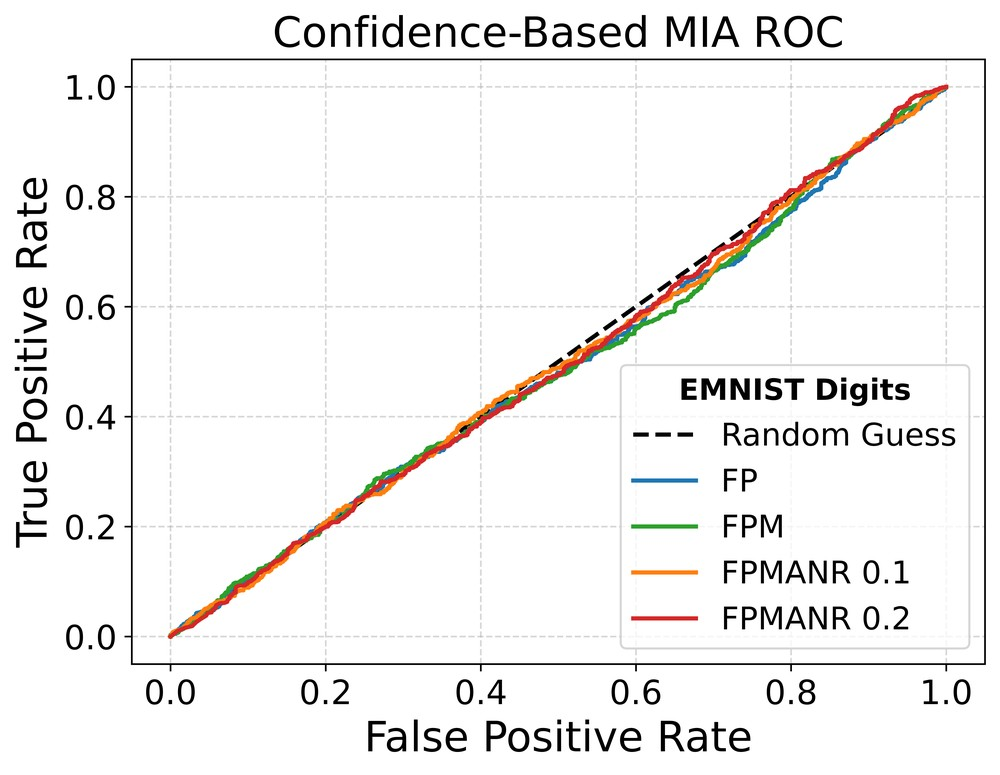
\includegraphics[width=0.32\textwidth]{figures/image67.jpg} & 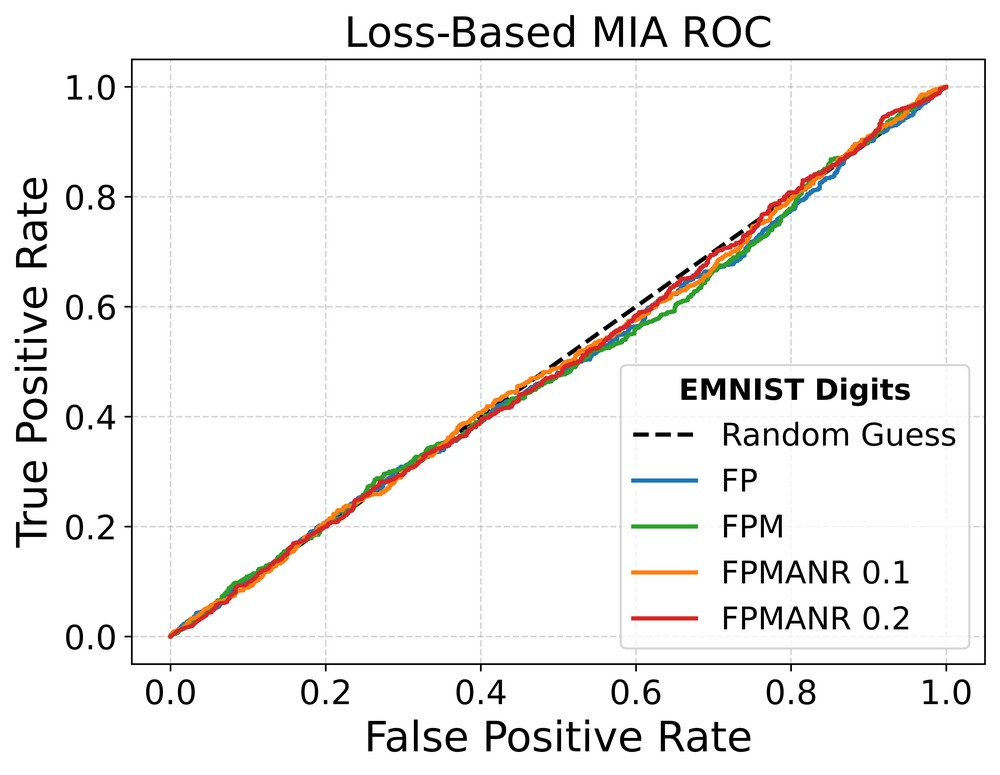
\includegraphics[width=0.32\textwidth]{figures/image68.jpg} & 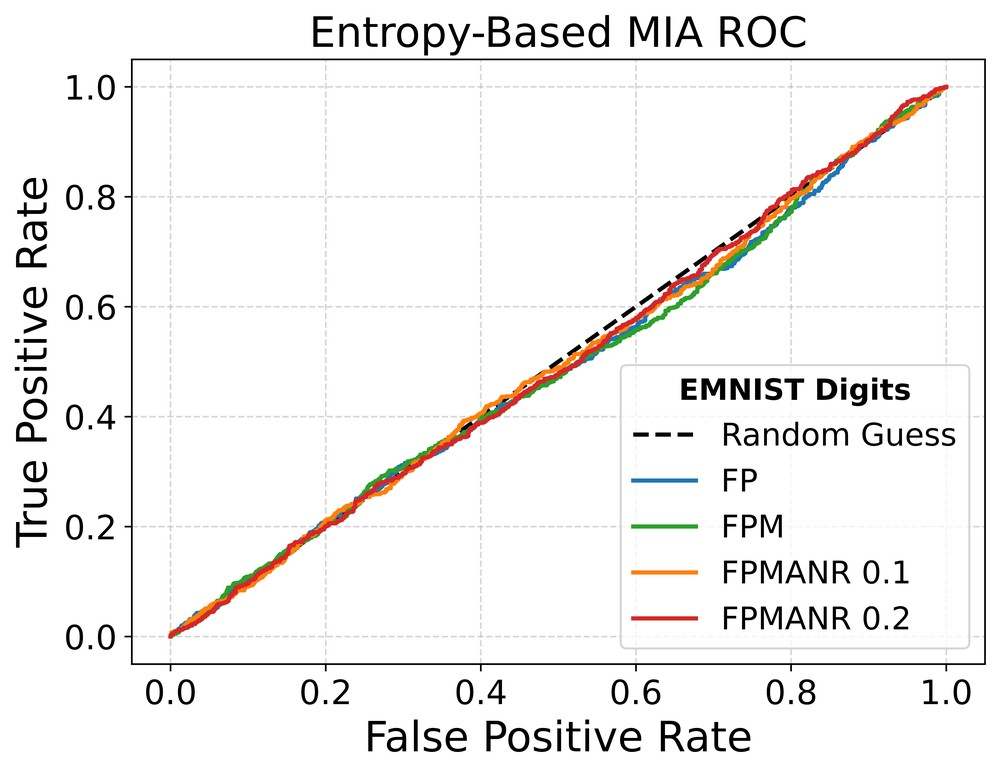
\includegraphics[width=0.32\textwidth]{figures/image69.jpg} \\
(i.a) & (i.b) & (i.c) \\
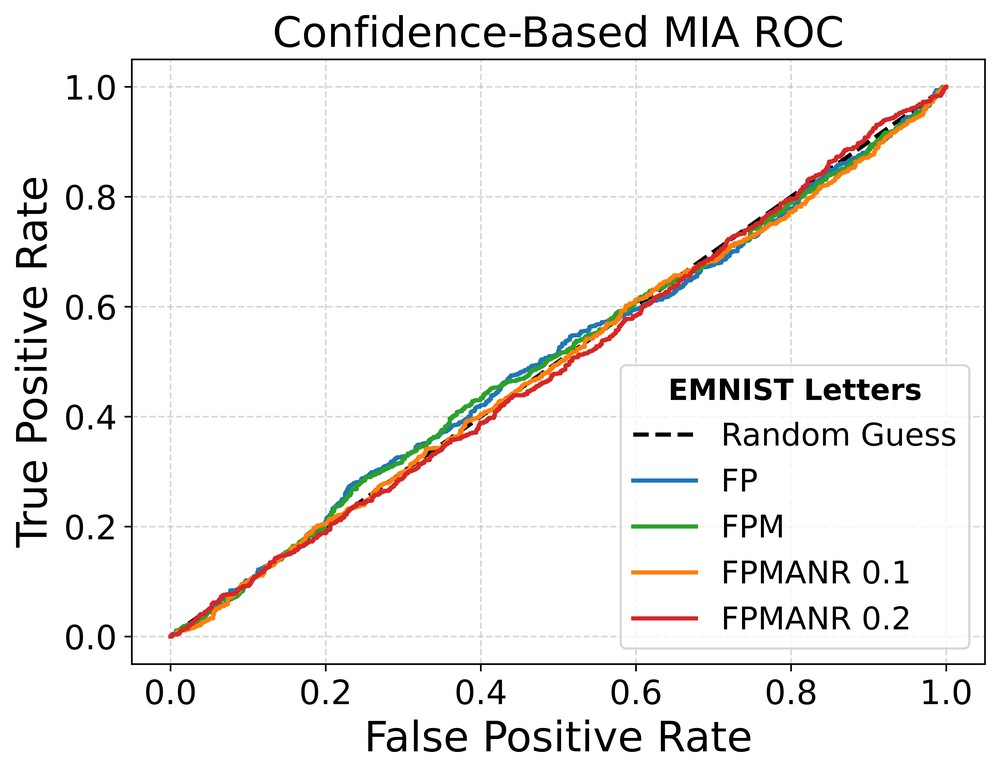
\includegraphics[width=0.32\textwidth]{figures/image70.jpg} & 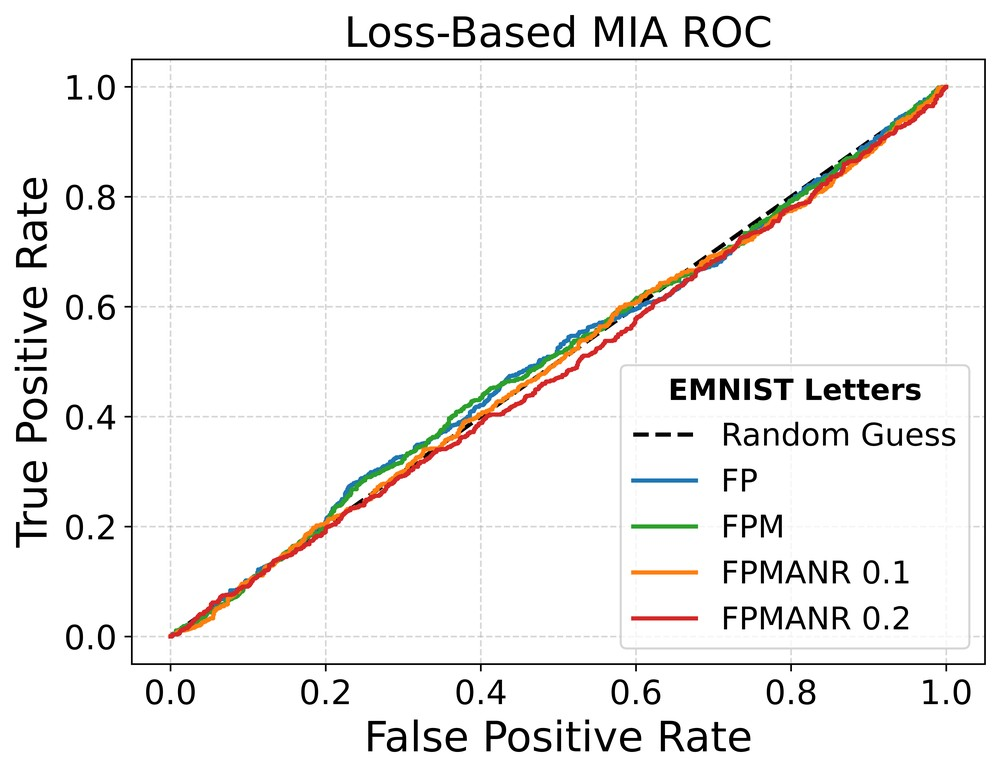
\includegraphics[width=0.32\textwidth]{figures/image71.jpg} & 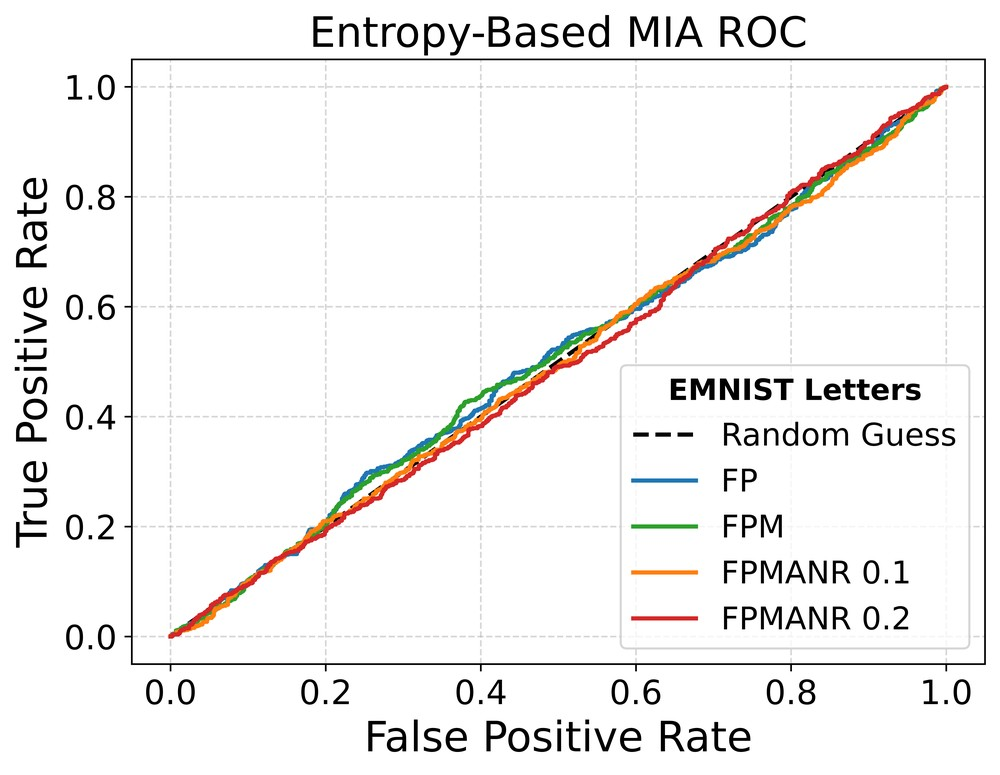
\includegraphics[width=0.32\textwidth]{figures/image72.jpg} \\
(ii.a) & (ii.b) & (ii.c) \\
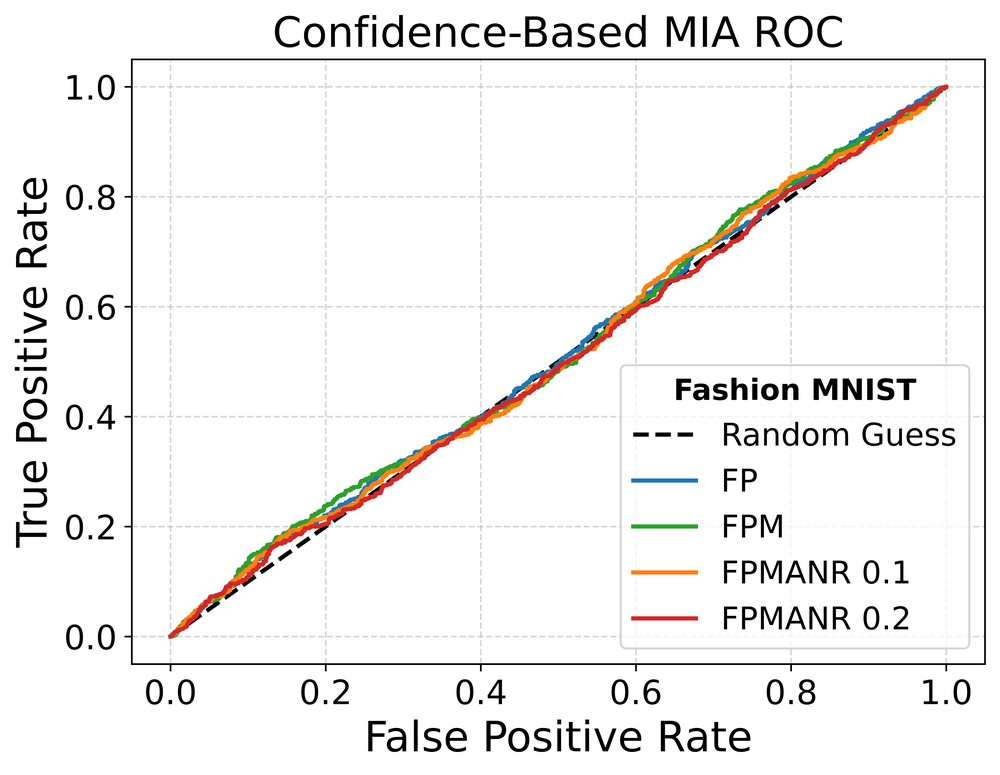
\includegraphics[width=0.32\textwidth]{figures/image73.jpg} & 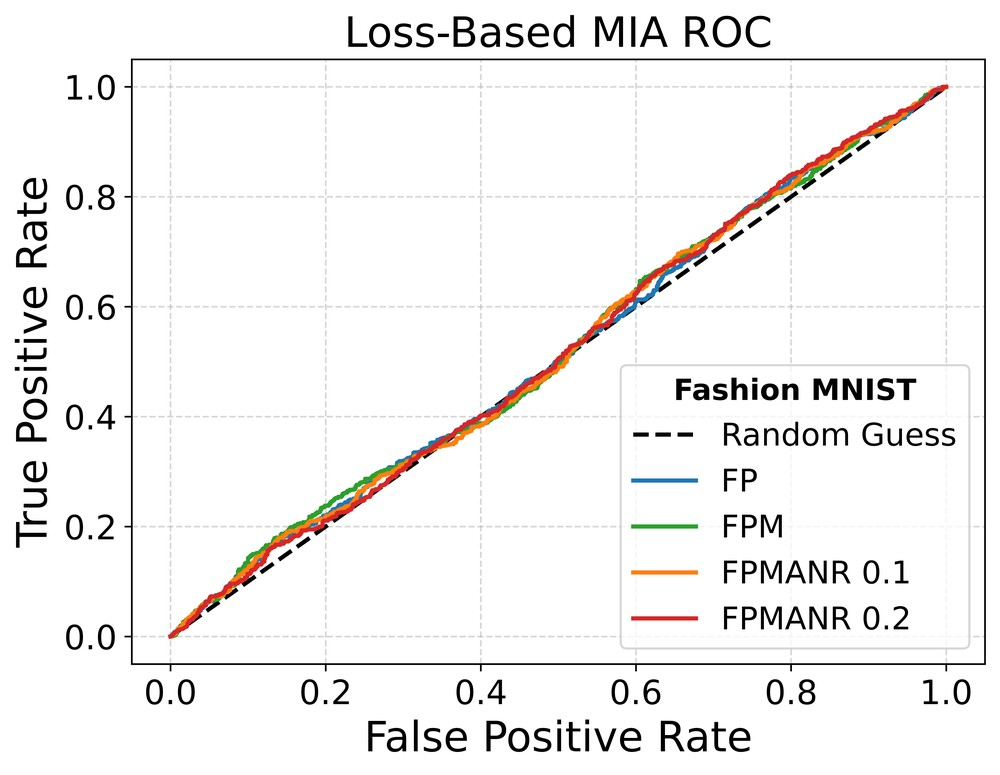
\includegraphics[width=0.32\textwidth]{figures/image74.jpg} & 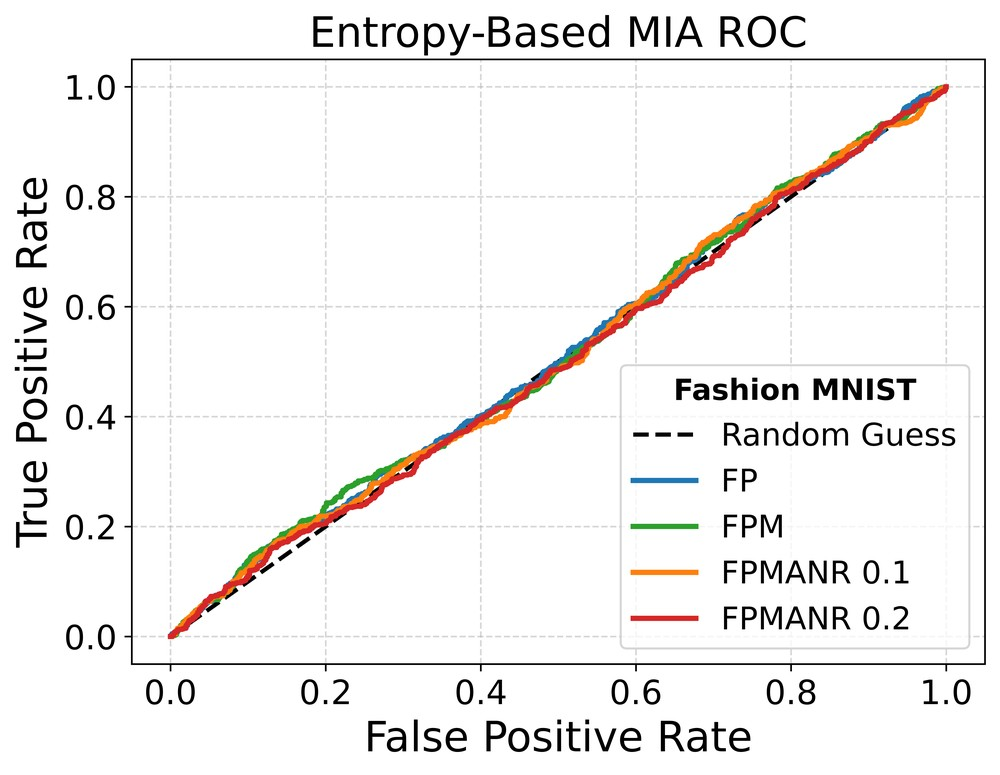
\includegraphics[width=0.32\textwidth]{figures/image75.jpg} \\
(iii.a) & (iii.b) & (iii.c) \\
\end{tabular}
\caption{ROC curves for MIAs under FP, FPM, FPMANR 0.1, and FPMANR 0.2 on (i) EMNIST Digits, (ii) EMNIST Letters, and (iii) Fashion-MNIST.}
\label{fig:4}
\end{figure*}

For EMNIST Digits, FP and FPM produce confidence, loss, and entropy AUC values around 0.49, with attack accuracies between 49.60\% and 50.15\%. The introduction of adaptive noise in FPMANR 0.1 and FPMANR 0.2 moves the AUC values slightly closer to 0.5, indicating that the attack becomes increasingly similar to random guessing. The corresponding attack accuracies also remain near 50\%, confirming that membership information is not effectively exposed through the shared updates.

A similar trend is observed for EMNIST Letters. FP and FPM achieve AUC values slightly above 0.50, whereas FPMANR 0.1 and FPMANR 0.2 reduce the confidence- and entropy-based AUC values toward 0.49--0.50. Although small fluctuations appear among different attack metrics, all results remain close to the random-guessing baseline, indicating weak membership inference capability.

For Fashion-MNIST, FP and FPM exhibit the highest AUC values among the three datasets, reaching approximately 0.51--0.52. However, these values are still very close to 0.5 and therefore provide only marginal advantage to the attacker. The addition of adaptive noise further reduces the confidence- and entropy-based AUC values, with FPMANR 0.2 achieving values closest to the random baseline. Attack accuracies also remain near 50\%, showing that the attacker gains little practical benefit from membership inference.

Overall, the ROC curves and quantitative results consistently indicate that MIAs are largely ineffective against all evaluated settings. Pairwise masking maintains a privacy level comparable to FP, while the addition of adaptive noise further reduces the distinguishability between member and non-member samples, pushing the attack performance closer to random guessing.

\begin{table*}
\centering
\scriptsize
\caption{MIA Performance Across Different Datasets and Model Configurations}
\label{tab:2}
\begin{tabular}{l l c c c c}
\toprule
\textbf{Dataset} & \textbf{Model} & \textbf{Confidence AUC $\downarrow$} & \textbf{Loss AUC $\downarrow$} & \textbf{Entropy AUC $\downarrow$} & \textbf{Attack Accuracy (\%) $\downarrow$} \\
\midrule
\multirow{4}{*}{EMNIST Digits} & FP & 0.4889 & 0.4893 & 0.4888 & 49.60\% \\
 & FPM & 0.4891 & 0.4892 & 0.4889 & 50.15\% \\
 & FPMANR 0.1 & 0.4943 & 0.4952 & 0.4941 & 50.15\% \\
 & FPMANR 0.2 & 0.4951 & 0.4952 & 0.4948 & 50.00\% \\
\midrule
\multirow{4}{*}{EMNIST Letters} & FP & 0.5033 & 0.5057 & 0.5027 & 48.60\% \\
 & FPM & 0.5041 & 0.5059 & 0.5033 & 49.20\% \\
 & FPMANR 0.1 & 0.4936 & 0.4955 & 0.4931 & 50.05\% \\
 & FPMANR 0.2 & 0.4947 & 0.4858 & 0.4927 & 49.45\% \\
\midrule
\multirow{4}{*}{Fashion-MNIST} & FP & 0.5119 & 0.5148 & 0.5106 & 50.05\% \\
 & FPM & 0.5126 & 0.5169 & 0.5111 & 50.90\% \\
 & FPMANR 0.1 & 0.5085 & 0.5145 & 0.5076 & 51.30\% \\
 & FPMANR 0.2 & 0.5004 & 0.5145 & 0.4997 & 49.40\% \\
\bottomrule
\end{tabular}
\end{table*}

Considering both privacy and model utility, FPMANR 0.1 provides the best balance among all evaluated settings. Compared with FP and FPM, it significantly reduces the effectiveness of gradient reconstruction attacks, driving the reconstruction success rate to nearly zero across all datasets while substantially lowering structural similarity and increasing perceptual distortion. At the same time, MIA performance remains close to random guessing, with AUC values near 0.5 and attack accuracies around 50\%. Although FPMANR 0.2 offers slightly stronger privacy in some cases, the additional improvement is relatively small compared with the noticeable reduction in classification performance. Therefore, FPMANR 0.1 is selected as the preferred configuration of the proposed framework, as it delivers strong resistance against privacy attacks while maintaining high model accuracy and training effectiveness.

\subsection{Dropout Recovery Validation}

This section evaluates whether the proposed recovery mechanism preserves correct mask cancellation when client dropouts occur. The residual mask norm is defined as $R = \left\| \sum_{i \in S}M_{i} \right\|$, where $M_{i}$ denotes the masking vector of active client $i$, and $S$ denotes the set of active clients in the communication round. A value close to zero indicates successful mask cancellation.

\xfig{fig:5} shows that the residual mask norm remains near zero in all rounds when the recovery mechanism is applied, even under client dropouts. Without recovery, nonzero residual masks appear whenever clients drop out, while the residual returns to near zero only when no dropout occurs. These results confirm that the proposed recovery mechanism preserves correct mask cancellation and aggregation consistency under varying client participation.

\begin{figure}
\centering
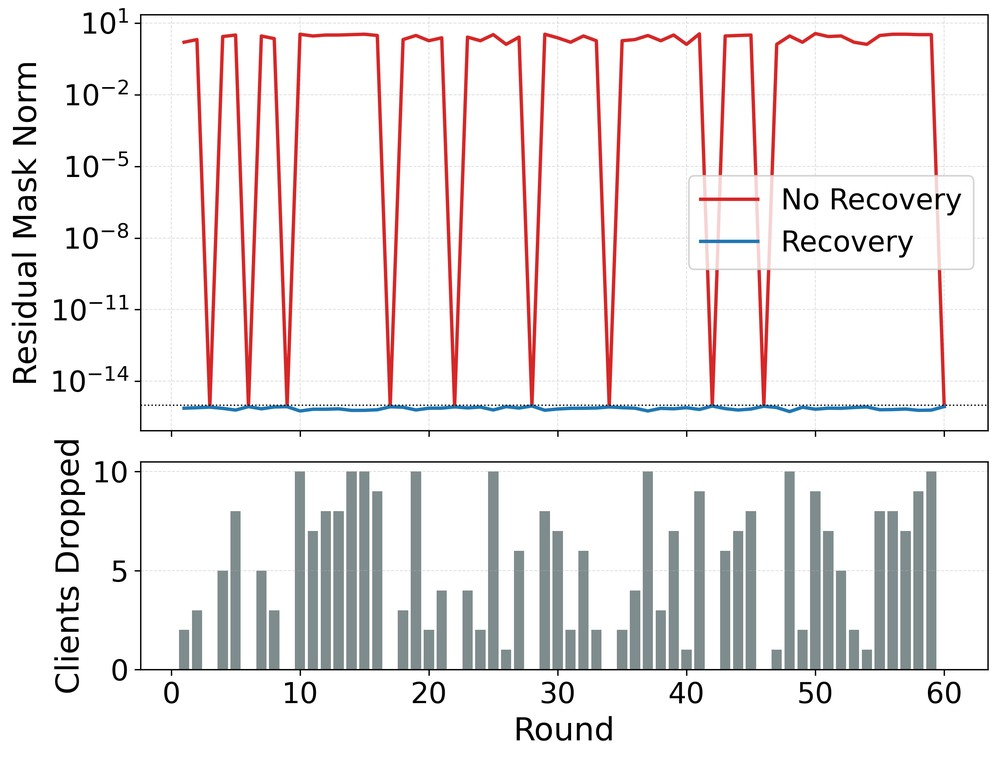
\includegraphics[width=0.95\columnwidth]{figures/image76.jpg}
\caption{Effect of the recovery mechanism on mask cancellation under client dropouts.}
\label{fig:5}
\end{figure}

\subsection{Comparison with Existing Methods}

This section presents a comparison of the proposed FPMANR framework with existing FL and privacy-preserving methods in terms of design characteristics and computational complexity.

\xtab{tab:3} shows that FPMANR integrates adaptive noise and pairwise masking to improve privacy protection while maintaining efficient communication and stable training under non-IID settings.

\begin{table*}
\centering
\tiny
\caption{Qualitative comparison of the proposed FPMANR framework with existing FL and privacy-preserving methods.}
\label{tab:3}
\begin{tabularx}{\textwidth}{>{\raggedright\arraybackslash}X >{\raggedright\arraybackslash}X >{\raggedright\arraybackslash}X >{\raggedright\arraybackslash}X >{\raggedright\arraybackslash}X >{\raggedright\arraybackslash}X >{\raggedright\arraybackslash}X >{\raggedright\arraybackslash}X >{\raggedright\arraybackslash}X}
\toprule
\textbf{Method} & \textbf{Privacy Mechanism} & \textbf{Masking Topology} & \textbf{Client Drift Control} & \textbf{Non-IID Support} & \textbf{Dropout Handling} & \textbf{Gradient Leakage Protection} & \textbf{MIA Resistance} & \textbf{Exact Aggregation} \\
\midrule
FedAvg \citep{mcmahan2017communication} & None & Centralized Star & \ding{55} & Partial & Fractional selection & \ding{55} & \ding{55} & \ding{51} \\
FedProx \citep{li2020federated} & None & Centralized Star & \ding{51} (Proximal Term) & \ding{51} & Partial work tolerated & \ding{55} & \ding{55} & \ding{51} \\
DP-SGD \citep{fernandez2025differential} & Fixed Global DP & Centralized Star & \ding{55} & Partial & Fractional selection & \ding{51} & \ding{51} & Perturbed \\
Adap DP-FL \citep{fu2022adap} & Adaptive Global DP & Centralized Star & \ding{55} & Partial & Fractional selection & \ding{51} & \ding{51} & Perturbed \\
ALDP-FL \citep{cui2025aldp} & Adaptive Local DP & Centralized Star & \ding{55} & Partial & Fractional selection & \ding{51} & \ding{51} & Perturbed \\
SecAgg \citep{bonawitz2017practical} & Cryptographic SMPC & All-to-all Mesh & \ding{55} & \ding{51} & Fault-tolerant recovery & \ding{51} & \ding{55} & \ding{51} \\
GVSA \citep{zhou2025group} & Crypto masking + Secret Sharing & Group-based & \ding{55} & \ding{51} & Group secret reconstruction & \ding{51} & \ding{55} & \ding{51} \\
\textbf{FPMANR (Proposed)} & \textbf{Hybrid (Adaptive Noise + Masking)} & \textbf{2-neighbor Ring} & \textbf{\ding{51} (Proximal Term)} & \textbf{\ding{51}} & \textbf{Ring repair + threshold} & \textbf{\ding{51}} & \textbf{\ding{51}} & \textbf{Perturbed} \\
\bottomrule
\end{tabularx}
\end{table*}

\xtab{tab:4} compares the asymptotic computation and communication complexities of the proposed FPMANR framework with existing FL and secure aggregation methods. The comparison shows that FPMANR maintains the computational and communication efficiency of conventional FL while reducing the communication overhead associated with large-scale masking-based aggregation schemes.

\begin{table*}
\centering
\footnotesize
\caption{Asymptotic complexity comparison of the proposed FPMANR framework and existing FL and secure aggregation methods.}
\label{tab:4}
\begin{tabular}{l c c c}
\toprule
\textbf{Method} & \textbf{User Computation} & \textbf{User Communication} & \textbf{Server Communication} \\
\midrule
FedAvg \citep{mcmahan2017communication} & O(E$\cdot$b$\cdot$m) & O(m) & O(n$\cdot$m) \\
FedProx \citep{li2020federated} & O(E$\cdot$b$\cdot$m) & O(m) & O(n$\cdot$m) \\
DP-SGD \citep{fernandez2025differential} & O(b$\cdot$m)\dag{} & O(m) & O(n$\cdot$m) \\
Adap DP-FL \citep{fu2022adap} & O(E$\cdot$b$\cdot$m) & O(m) & O(n$\cdot$m) \\
ALDP-FL \citep{cui2025aldp} & O(E$\cdot$b$\cdot$m) & O(m) & O(n$\cdot$m) \\
SecAgg \citep{bonawitz2017practical} & O(n+m) & O(n+m) & O(n$^{2}$+n$\cdot$m) \\
GVSA \citep{zhou2025group} & O(g+m) & O(g+m) & O(n$\cdot$g+n$\cdot$m) \\
\textbf{FPMANR (Proposed)} & \textbf{O(E$\cdot$b$\cdot$m)} & \textbf{O(m)} & \textbf{O(n$\cdot$m)} \\
\bottomrule
\end{tabular}
\par\vspace{2pt}\begin{minipage}{\textwidth}\footnotesize
\dag{} DP-SGD performs gradient clipping and noise addition at the mini-batch level; therefore, its computational complexity is expressed in terms of the batch size $b$ rather than the epoch count $E$.

Here, $n$ denotes the number of active clients, $m$ the number of model parameters, $b$ the mini-batch size, $E$ the number of local epochs, and $g$ the group size.
\end{minipage}
\end{table*}

\section{Conclusion}
\label{sec:7}

FPMANR combines FedProx for local training, two-neighbor pairwise masking in a ring topology, adaptive layer-wise Gaussian noise, and a client dropout recovery mechanism to protect individual updates and enhance privacy in FL under non-IID data. Experiments on the EMNIST Digits, EMNIST Letters, and Fashion-MNIST datasets show that pairwise masking preserves training performance with only small computational overhead, while adaptive Gaussian noise provides additional privacy protection with a moderate reduction in model accuracy. On EMNIST Digits, FPM achieves 98.40\% validation accuracy and 98.52\% test accuracy, while FPMANR 0.1 achieves 98.02\% validation accuracy and 98.10\% test accuracy, and FPMANR 0.2 achieves 96.35\% validation accuracy and 96.57\% test accuracy. On EMNIST Letters, FPMANR 0.1 and FPMANR 0.2 achieve test accuracies of 85.39\% and 73.37\%, respectively, while on Fashion-MNIST they achieve 74.51\% and 73.12\%. The results show a clear privacy--utility trade-off, where adaptive noise improves privacy but slightly reduces accuracy. Visual and quantitative evaluations using DLG, iDLG, and GradInv attacks show that FP reveals recognizable information, while FPM reduces reconstruction quality and FPMANR further produces highly distorted and unrecognizable reconstructions, with reconstruction success rates close to zero in most cases. MIAs also remain close to random guessing across all datasets, with AUC values around 0.5 and attack accuracies near 50\%, indicating limited membership leakage. Among the evaluated settings, FPMANR 0.1 provides the best balance between privacy and utility by significantly reducing gradient leakage while maintaining high classification performance. Overall, FPMANR provides a practical and attack-resistant FL framework that maintains stable training under heterogeneous client data distributions while protecting local updates using adaptive noise and pairwise masking. The proposed recovery mechanism further ensures robust aggregation under client dropouts without requiring local retraining. Future work includes evaluating FPMANR on larger-scale FL environments and additional real-world datasets, testing against a wider range of privacy and security attacks, and exploring stronger formal privacy guarantees while further improving the privacy--utility trade-off.

\bibliographystyle{cas-model2-names}
\bibliography{references}

\end{document}